%% Chapter 10 — 추론 최적화
\setcounter{chapter}{9}
\chapter{추론 최적화}
\chaptersubtitle{메모리 벽, 양자화, 그래프 컴파일 — 같은 GPU를 절반의 비용으로}

\begin{calloutbox}{tbbblue}{tbbbluefill}
{\normalsize\bfseries\color{tbbblue}학습 목표}\par\vspace{3pt}
\begin{tbbitemize}
  \item 한 장의 4열 비용표를 바탕으로, 서빙에서 "최적화"란 \textbf{같은 답을 요청당 더 낮은 비용으로 제공하는 것}임을 설명한다. 가장 큰 개선에 새 하드웨어도 새 모델도 필요하지 않았던 이유도 이해한다.
  \item 두 줄짜리 산술 집약도 추정으로 워크로드가 \textbf{메모리 벽}의 어느 쪽에 있는지 진단하고, 어떤 최적화가 효과를 내고 어떤 최적화가 기대에 못 미칠지 예측한다.
  \item 스케일, 영점, 채널별 세분성, 보정이라는 양자화의 작동 원리를 설명하고, 학습과 달리 추론이 거친 눈금을 견디는 이유를 이미 익숙한 JPEG 사례와 연결해 이해한다.
  \item \textbf{PTQ 워크플로}를 처음부터 끝까지 실행하고 엔지니어답게 게이트를 적용한다. 작업 지표와 명시된 허용 오차를 비교하고, 슬라이스를 점검하며, 기존 산출물을 제자리에서 바꾸지 않고 다이제스트에 고정된 새 산출물을 만든다.
  \item ONNX Runtime, TensorRT, torch.compile에서 \textbf{그래프 컴파일러}가 제공하는 이점(융합, 폴딩, 레이아웃 계획, 오토튜닝)과 그 대가(적용 범위의 제약, 빌드 시간, 워밍업)를 설명한다.
  \item 컴파일, 양자화, 배치라는 수단을 올바른 순서로 조합하고, 제9장의 t(B) = a + b·B를 다시 적합해 개선의 출처를 입증한 뒤 프로젝트에 필요한 전후 벤치마크 보고서를 완성한다.
\end{tbbitemize}
\end{calloutbox}

\vspace{3.5pt}

\begin{calloutbox}{tbbteal}{tbbtealfill}
{\normalsize\bfseries\color{tbbteal}핵심 용어}\par\vspace{3pt}
요청당 비용 · 메모리 벽 · 산술 집약도 · 루프라인 · 고정 메모리와 PCIe · 양자화 · FP16 / BF16 / FP8 / INT8 / INT4 · 스케일과 영점 · 채널별 / 그룹별 · 보정(최솟값–최댓값, 백분위수, KL) · PTQ 대 QAT · 활성값 이상치 · 게이트(정확도 허용 오차) · 커널 융합 · 상수 폴딩 · 오토튜닝 · ONNX Runtime EP · TensorRT 엔진 · torch.compile · 형상 프로파일 · 패딩과 버킷팅
\end{calloutbox}

\vspace{3.5pt}

\begin{calloutbox}{tbblightgray}{tbbboxfill}
{\normalsize\bfseries\color{tbbink}장 구성}\par\vspace{3pt}
\textbf{10.1} 하나의 모델, 네 가지 비용 — 이미 살아가는 손실 압축의 세계    \textbf{10.2} 메모리 벽: 최적화보다 진단이 먼저다    \textbf{10.3} 양자화: 더 거친 눈금, 정직한 게이트    \textbf{10.4} 그래프 컴파일: 더 적은 왕복과 실행    \textbf{10.5} 수단 조합하기 — a와 b 다시 적합하기    \textbf{10.6} 실습: 전후 벤치마크 보고서 — 이어서 요약, 연습문제, 더 읽을거리
\end{calloutbox}

\section{하나의 모델, 네 가지 비용 — 이미 살아가는 손실 압축의 세계}

제7장은 \$900라는 상한 앞에 월 \$4,762라는 청구서를 내놓고, 그 격차 자체가 앞으로 배울 내용이라고 예고했다. 제9장에서는 하나의 레플리카가 정직하게 동작하도록 만들었다. 이번 장은 그 약속을 처음으로 크게 갚는다. 이번 주를 규정하는 다음 사례부터 살펴보자. 프로젝트의 같은 모델을, 플릿이 임대한 같은 L4와 같은 SLO 및 Locust 스윕 아래 네 가지 방식으로 서빙한 결과다.

\begin{terminalbox}
\begin{Verbatim}[breaklines=true,breakanywhere=true,fontsize=\small,formatcom=\color{tbbtermfg},codes=\tbbcodeactive]
# the project's 3B chat model. same L4, same SLO (p99<=500ms),
# same open-loop sweep (§9.5). only the execution stack changes:
  stack                p99@peak   req/s@SLO   $/M req    vs
  A eager FP32         -- 12 GB weights + KV cache + activations:
                          OOM at peak load on the 24 GB card --
  B eager FP16          492ms       28/s       $7.94     1.0x
  C + ONNX Runtime      455ms       39/s       $5.70     1.4x
  D + TensorRT FP16     448ms       46/s       $4.83     1.6x
  E + TensorRT INT8     461ms       57/s       $3.90     2.0x
# same weights (within a gated tolerance - §10.3), same GPU.
# the fleet: 200 req/s / 57 = 4 replicas = $2,381/mo. as promised.
\end{Verbatim}
\end{terminalbox}
\figcaption{사례 10-A  하나의 모델, 네 가지 비용. B행에서 E행으로 가는 동안 모델의 지식은 전혀 바뀌지 않았지만 비용은 절반이 되었다. A행도 별도의 교훈을 준다. 정밀도는 속도의 문제이기 전에 모델이 메모리에 들어가기나 하는가의 문제다.}

작동 원리를 보기 전에 이 사례가 주는 세 가지 교훈을 읽어 보자. 첫째, 여기서 \textbf{"최적화"란 같은 SLO에서 요청당 비용을 낮추는 것}이다. 실제로는 아무도 서빙하지 않는 배치 512의 과시용 벤치마크가 아니라, §9.5의 정직한 수치를 각 행마다 다시 측정했다. 제1장에서 기법이라면 그래야 한다고 했듯 서빙 삼각형 자체가 \textit{이동}하고 있다. 둘째, \textbf{개선 효과는 합성된다}. C는 컴파일러 패스, D는 더 깊은 컴파일러, E는 컴파일러 \textit{내부}에 양자화를 추가한다. 각 행은 이전 행의 개선을 그대로 이어받는다(§10.5에서 이 합성을 정식화한다). 셋째, \textbf{E행의 별표가 이 규율의 전부다}. INT8의 답은 FP16의 답과 비트 단위로 같지 않다. 하지만 \textit{벤치마크 전에 누군가 명시한 허용 오차 안에서는 동등}하다. 이는 이 장에서 SLO 문장에 대응하는 원칙이자, 엔지니어링과 막연한 기대를 가르는 기준이다(§10.3의 게이트).

\begin{tbbfigure}
  \adjustbox{max width=0.94\linewidth,max totalheight=0.46\textheight}{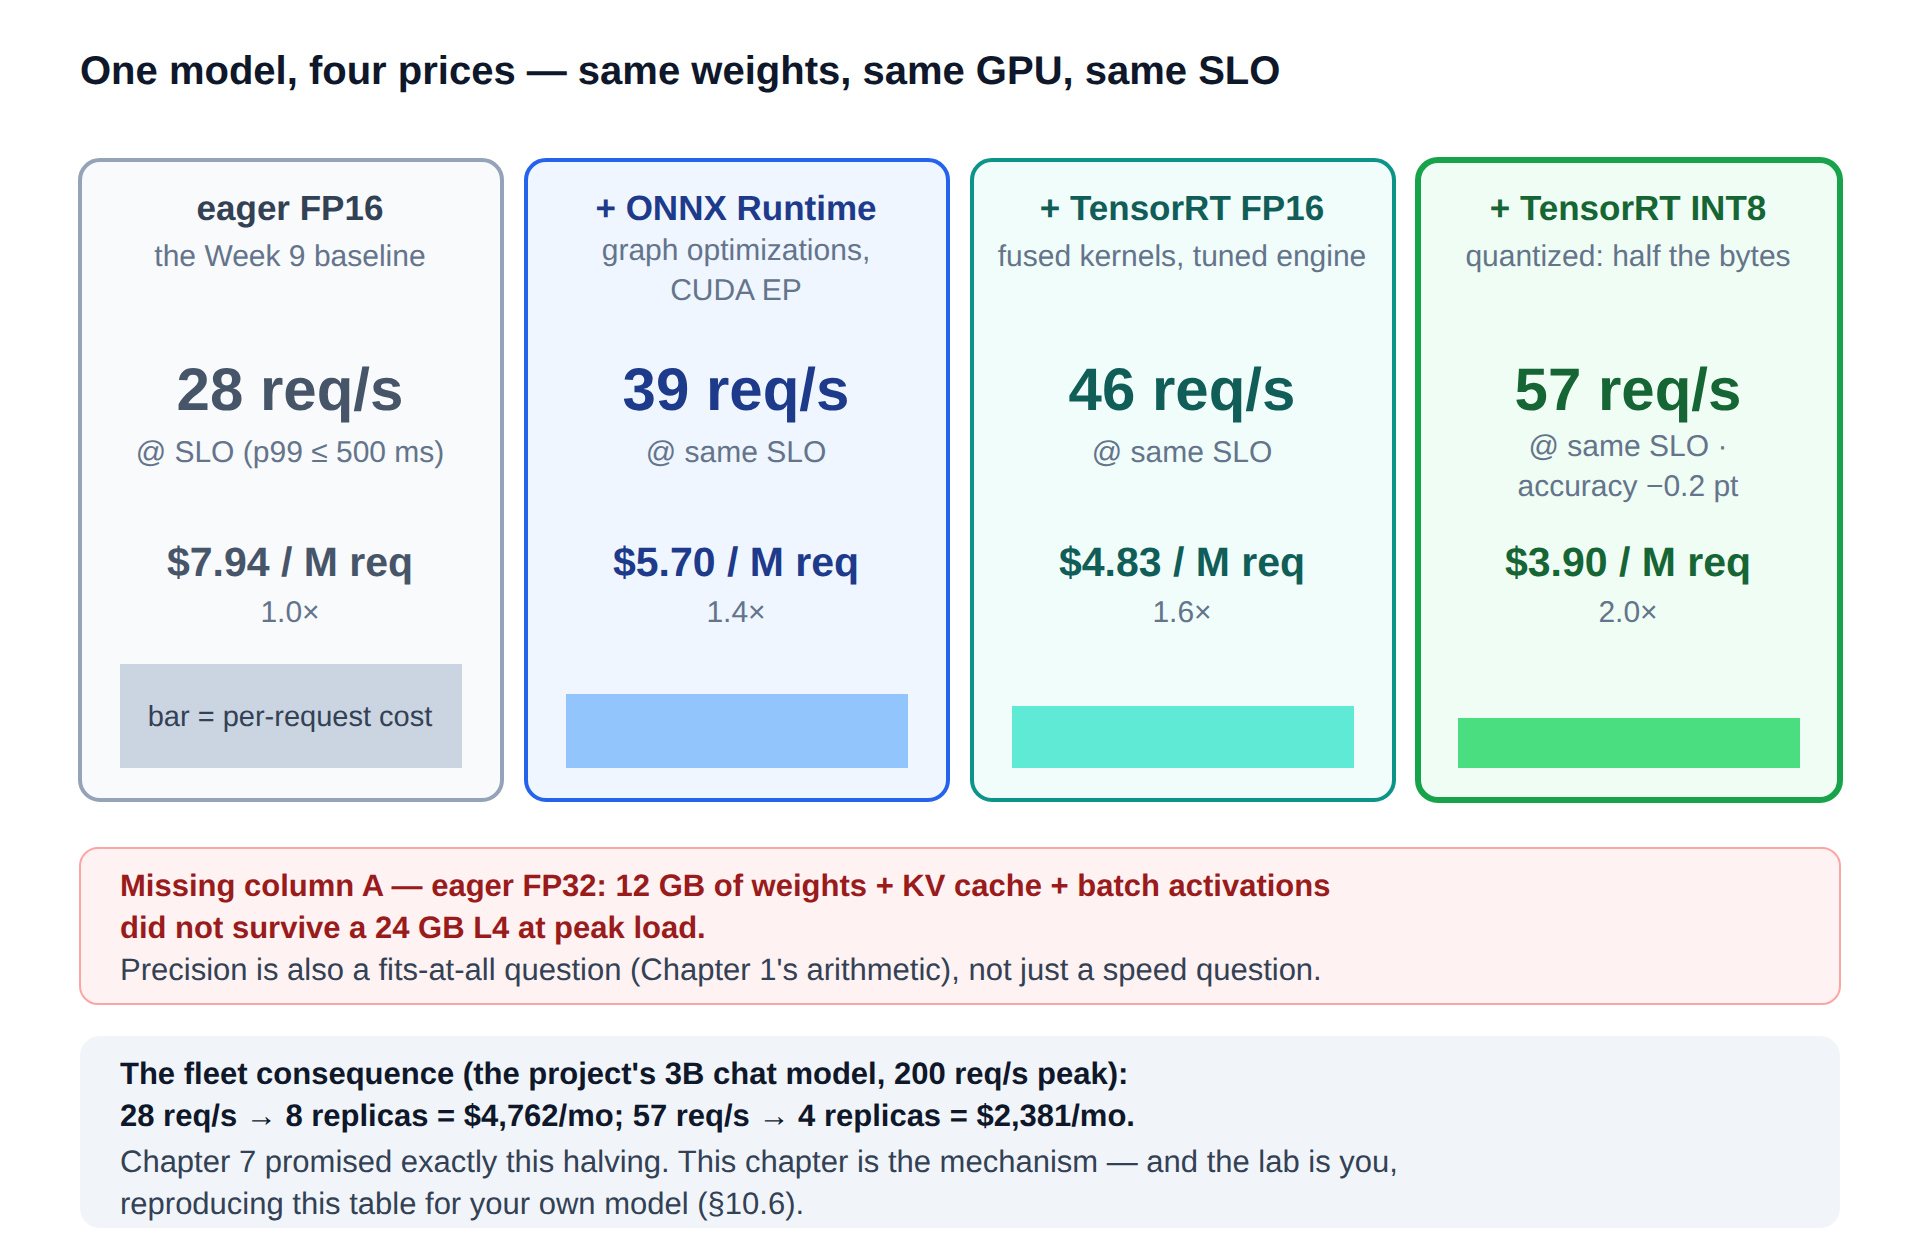
\includegraphics{figures/fig10-1_fourprices.png}}\\[3pt]
  \figcaption{그림 10-1  사례 10-A를 도식화한 모습. 같은 실리콘에서 달러당 유효 처리량이 2×가 되었다. 제7장이 예고한 플릿의 결과도 그대로 나타난다. 레플리카 8개가 4개로, \$4,762가 \$2,381로 줄었다.}
\end{tbbfigure}

\subsection*{우리는 평생 손실 압축을 믿고 살아왔다}

정밀도를 버리고도 결과물을 유지할 수 있다는 생각은 무모하게 들린다. 그러나 \textbf{우리가 감각으로 소비하는 세계 전체가 이미 이 원리 위에 세워져 있다}. 전화망이 음성을 디지털화했을 때(Bell System의 T1 반송파, 1962), 원음 그대로를 전송하지 않았다. 사람의 귀는 절대적인 간격보다 비율에 민감하므로 로그 눈금(μ-law 컴팬딩)의 \textbf{8-bit} 표본을 보냈다. 연속적인 아날로그 신호를 256단계로 줄였지만, 적절히 배치한 8비트만으로도 음성처럼 들렸다. 통화 속 어머니의 목소리가 잘못 들리는 일은 없었다. 30년 뒤에는 \textbf{JPEG (1992)}가 이미지에 같은 원리를 적용했다. 눈이 거의 감지하지 못하는 고주파 세부를 버려 바이트를 10분의 1로 줄여도 휴가 사진은 멀쩡했다. \textbf{MP3 (1993)}도 귀가 다른 소리에 가려 듣지 못하는 부분을 모델링해 음악에 이를 적용했다. 패턴은 언제나 같다. \textit{신호의 소비자가 실제로 필요한 것을 찾아내고, 나머지에는 비용을 쓰지 않는다.}

양자화는 이 패턴을 신경망에 적용한다. 단, 한 가지 멋진 치환이 있다. 여기서 "소비자"는 눈이나 귀가 아니라 \textbf{모델 자체의 결정}이다. 학습에는 실제로 높은 정밀도가 필요하다. 경사 하강법은 가중치를 10⁻⁵ 단위로 조금씩 움직이고 수백만 단계에 걸쳐 이를 누적한다. 그 작은 변화를 반올림해 없애면 학습이 멈춘다. 반면 추론에서 살아남아야 하는 것은 \textit{출력}뿐이다. 최댓값의 위치, 순위, 생성된 토큰이 유지되면 된다. 학습된 네트워크는 놀라울 만큼 관대한 소비자다. 좋은 최솟값 주변의 곡면은 평평해 모든 가중치를 몇 분의 1퍼센트 움직여도 손실이 거의 변하지 않고, 활성값에는 어차피 잡음이 있으며, 결정 경계에는 여유가 있다. 가중치 0.087231을 0.0872로 반올림하는 변화는 네트워크가 이미 무시하는 잡음보다 훨씬 작다. \textbf{대부분의 추론에서 FP32를 쓰는 것은 전화 통화에 스튜디오 마스터 음원을 보내는 것과 같다.} §10.3에서는 Bell Labs가 했던 만큼 세심하게 μ-law 변환을 수행한다. 신호를 측정하고 눈금을 잘 배치한 다음, \textit{듣는 사람이 차이를 알아채지 못하는지 검증한다}.

작동 원리로 들어가기 전에 이 장 전체를 조직하는 틀을 하나 더 세우자. 제9장은 두 매개변수 법칙 \textbf{t(B) = a + b·B}를 남겼다. a는 패스마다 드는 고정 비용(실행, 스케줄링, 가중치 스트리밍)이고, b는 항목마다 추가되는 한계 비용(연산)이다. 이번 장은 두 상수를 정조준한다. \textbf{컴파일은 a를 줄인다}(§10.4: 커널을 융합하고 상수를 폴딩하며, 활성값이 메모리를 불필요하게 왕복하지 않게 한다). \textbf{양자화는 b를 줄이고 a의 일부도 줄인다}(§10.3: 가중치당 바이트가 절반이면 각 패스의 가중치 스트리밍 부분도 절반이 된다). §10.2는 두 문장에 \textit{바이트}가 계속 등장하는 이유를 설명한다. 대부분의 추론에서 병목은 GPU의 연산 성능이 아니기 때문이다.

\begin{calloutbox}{tbbpurple}{tbbpurplefill}
{\normalsize\bfseries\color{tbbpurple}생각해 보기}\par\vspace{3pt}
\begin{tbbitemize}
  \item 사례 10-A의 A행에서 OOM 계산을 재구성하라. 3B params × 4 bytes = 12 GB의 가중치가 24 GB L4에 올라간다. 최대 부하에서 VRAM을 요구하는 다른 요소(배치 활성값, 채팅 모델의 시퀀스별 KV 캐시 — 제1장의 메모리 이야기와 제9장의 max\_batch\_size 상한)를 차례로 살펴보고, FP16 (6 GB)이 같은 서버에 여유를 준 이유를 설명하라.
  \item μ-law 비유에는 한계가 있다. 전화 통화의 품질은 조금 더 흐릿한 목소리처럼 점진적으로 나빠지지만, 분류기는 어느 순간 결정이 불연속적으로 뒤집힐 수 있다. 바로 이 차이 때문에 존재하는 §10.3의 안전장치는 무엇인가? 방송 엔지니어링에도 이에 해당하는 장치가 있는가?
  \item C행(ONNX Runtime)은 정밀도를 바꾸지도 양자화하지도 않고 1.4×의 개선을 얻었다. 제9장에서 배운 a와 b를 바탕으로 볼 때 이 개선은 어디에서 나왔어야 하는가? §10.4의 여러 메커니즘 중 가장 유력한 것은 무엇인가?
\end{tbbitemize}
\end{calloutbox}

\section{메모리 벽: 최적화보다 진단이 먼저다}

이 장의 모든 최적화 이야기는 현대 가속기의 화려하지 않은 사실 하나에 기대고 있다. \textbf{연산 속도가 빨라진 속도를 바이트가 가까워지는 속도가 따라가지 못했다.} T4는 초당 65조 회의 FP16 연산을 수행할 수 있지만, 같은 시간에 메모리가 공급할 수 있는 데이터는 320기가바이트뿐이다. 둘을 나누면 이 장치의 성격이 드러난다. 연산 장치가 굶지 않으려면 가져오는 \textbf{바이트당 약 200회의 부동소수점 연산}이 필요하다. 이 비율이 \textit{메모리 벽}이다. 이 이름은 1995년 Wulf와 McKee가 CPU 속도는 해마다 \textasciitilde{}50\%씩 늘지만 메모리 접근 성능은 \textasciitilde{}7\%만 개선된다는 사실을 발견하고, 업계가 전속력으로 벽을 향해 달리고 있다고 유명한 짧은 논문에서 경고하며 붙였다. GPU는 막대한 대역폭으로 충돌을 늦췄지만(HBM은 메모리 벽에 바치는 몸값이다), 그 비율은 계속 악화되었다. 워크로드가 벽의 어느 쪽에 있는지를 알면 벤치마크를 하기도 전에 어떤 최적화가 효과를 낼지 판단할 수 있다.

진단에 필요한 것은 하나의 수치다. \textbf{산술 집약도(AI), 즉 이동한 바이트당 수행한 FLOP 수}다. AI가 장치의 비율보다 큰 워크로드는 \textbf{연산 병목}이다. 다이가 실제로 바쁘므로 연산 자체를 더 저렴하게 만드는 것만 도움이 된다. 반대로 그 비율보다 낮으면 \textbf{메모리 병목}이다. 텐서가 흘러들어오는 동안 연산 장치는 쉬고 있으므로 "더 빠른 연산"은 아무것도 바꾸지 못하며, 오직 \textit{더 적은 바이트}만 효과가 있다. 그림 10-2는 이를 고전적인 \textbf{루프라인(roofline)}으로 나타낸다. 기울어진 대역폭 지붕과 평평한 연산 지붕이 있고, 둘이 만나는 능선이 있다. 서빙에는 불편한 소식이 있다. \textbf{서빙에 적합한 배치 크기에서 대부분의 추론은 능선 왼쪽}, 즉 메모리 병목 영역에 놓인다. 배치 1의 LLM 토큰 생성은 극단적인 사례다. 토큰 하나마다 모든 가중치를 다시 스트리밍해 각각 몇 번의 FLOP만 수행하므로 AI ≈ 1–10에 불과하고, 대역폭 병목에서 벗어날 가망이 없다. 이것이 제11장 전체의 난제다. 큰 배치의 CNN과 규모가 큰 GEMM만 연산 지붕에 도달한다.

\begin{tbbfigure}
  \adjustbox{max width=0.94\linewidth,max totalheight=0.46\textheight}{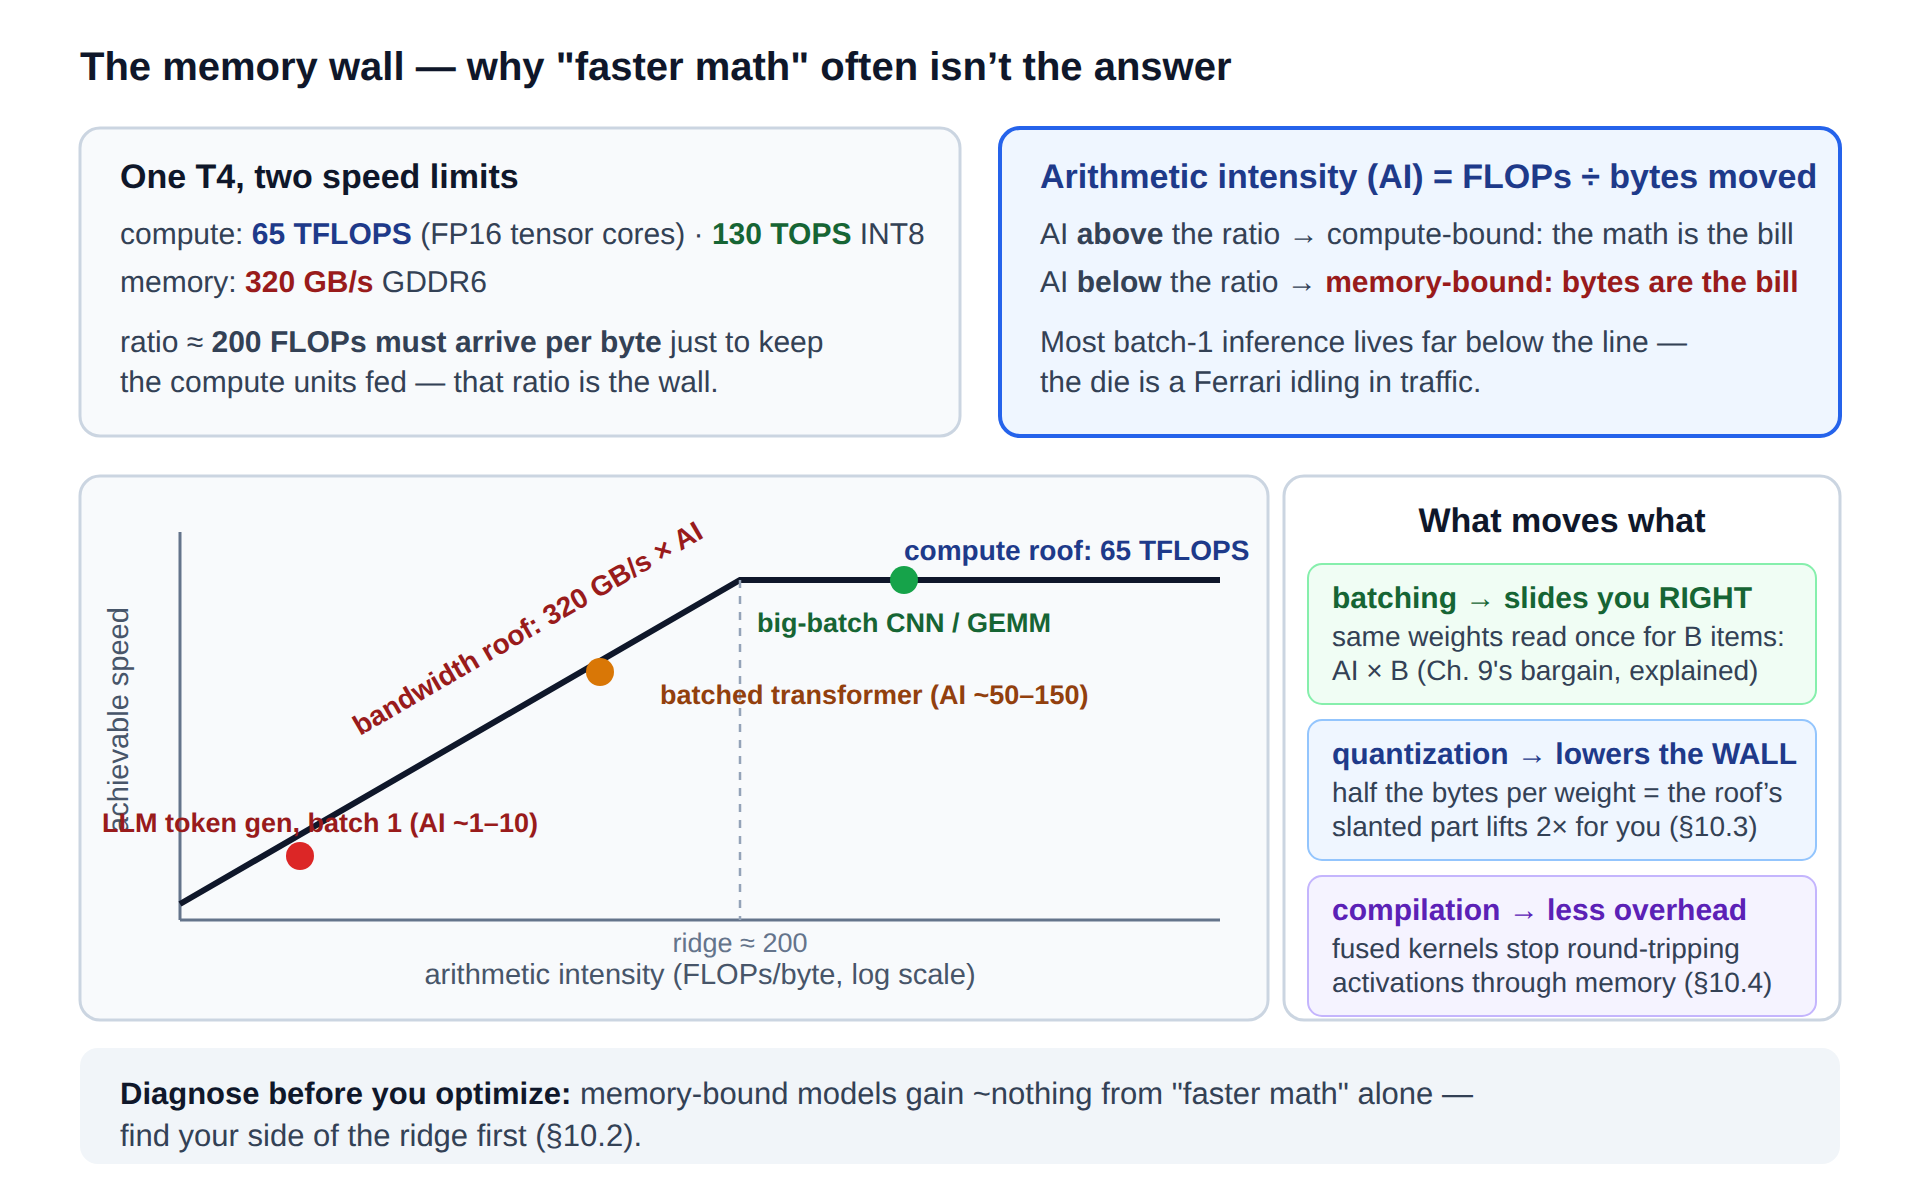
\includegraphics{figures/fig10-2_memorywall.png}}\\[3pt]
  \figcaption{그림 10-2  루프라인으로 표현한 메모리 벽. 배치는 오른쪽으로 이동시킨다(같은 가중치로 바이트당 더 많은 작업을 수행한다). 양자화는 기울어진 지붕을 들어 올린다(가중치당 바이트가 줄어든다). 컴파일은 불필요한 왕복을 없앤다. 먼저 진단하라. 무엇이 효과를 낼지는 능선이 결정한다.}
\end{tbbfigure}

\subsection*{능선 적용하기: 이미 다뤄 본 세 가지 워크로드}

2주 차부터 실행해 온 세 연산의 AI를 직접 계산하면 이 정의는 곧 직관이 된다. 숫자를 모두 펼쳐서 계산해 보자. \textbf{첫째, 토큰을 생성하는 행렬–벡터 곱이다.} 어떤 트랜스포머 계층의 FP16 가중치 행렬이 4,096 × 4,096이라면 크기는 33.6 MB다. 입력 벡터 하나를 곱할 때 2 × 4,096² ≈ 33.6 MFLOP을 수행한다. 둘을 나누면 \textbf{AI ≈ 바이트당 1 FLOP}이다. 가중치를 한 번 읽어 한 번 쓴다. 능선이 200인 장치에서 이는 워크로드라기보다 약간의 연산을 곁들인 바이트 배달 서비스다. 이제 B개의 요청을 배치로 묶자. 같은 33.6 MB의 가중치가 B개의 벡터를 처리하므로 FLOP은 B배가 되지만 바이트는 거의 변하지 않는다. 따라서 \textbf{AI ≈ B}다. 이 한 줄이 배치 처리의 이론 전체이며, 뒤에 나올 표 10-3의 핵심이기도 하다. T4의 능선에 닿으려면 B ≈ 200이어야 한다. 하지만 SLO 때문에 이 모델의 배치는 약 32가 상한이므로 생성은 늘 메모리 병목 영역에 \textit{머문다}. 제11장의 첫 문제가 여기서는 산술로 드러난다.

\textbf{둘째, ReLU}다. max(0, x)는 원소마다 한 번의 FLOP을 수행한다. FP16 원소 하나를 읽고(2 bytes) 써야 하므로(2 bytes) \textbf{AI = 1 ÷ 4 = 0.25}이며, 능선보다 800배 낮다. 지금껏 만들어진 어떤 하드웨어도 원소별 연산을 메모리 속도보다 빠르게 실행하지 못한다. 그래서 §10.4의 컴파일러는 ReLU에 별도 커널을 주지 않는다. 값을 만드는 연산과 융합하면 그 바이트 자체가 사라진다. \textbf{셋째, 실제 합성곱}을 보자. 56×56 특징 맵에서 3×3, 64→64 채널인 연산이다. FLOP은 2 × 9 × 64 × 64 × 56² ≈ 231 M이다. 바이트는 입력 0.40 MB + 가중치 0.07 MB + 출력 0.40 MB ≈ 0.88 MB다. 따라서 \textbf{AI ≈ 264}로 T4의 능선 \textit{바로 위}에 놓인다. 합성곱은 3,136개 공간 위치 전체에서 각 가중치를 재사용한다. 데이터 재사용이 연산 자체에 내장되어 있다. 이 때문에 CNN은 루프라인의 모범 시민이고, 9주 차 분류기의 개선은 가중치 스트리밍보다 연산 속도와 실행 오버헤드에서 나온다. 같은 GPU가 한 모델에서는 굶고 다른 모델에서는 땀을 흘리는 이유도 여기에 있다.

세 수치 \textbf{≈ B, 0.25, 264}를 머릿속에 두자. 앞으로 서빙할 거의 모든 계층은 이 셋 중 하나가 다른 옷을 입은 모습이다. 첫 진단에는 프로파일러도 필요 없다. 두 줄의 계산이면 충분하며, 실습 보고서도 바로 이 두 줄로 시작해야 한다.

\begin{terminalbox}
\begin{Verbatim}[breaklines=true,breakanywhere=true,fontsize=\small,formatcom=\color{tbbtermfg},codes=\tbbcodeactive]
# is my model memory-bound at this batch size? no profiler needed.
# the project's 3B chat model, on the fleet's L4 (24 GB, 300 GB/s):
# floor set by BYTES: weights must stream once per forward pass:
$ python -c "print(6.0e9 / 300e9 * 1e3, 'ms floor per pass')"
20.0 ms floor per pass      # 3B params x 2B (FP16) / 300 GB/s
# floor set by MATH: ~2 FLOPs/param/item -> batch 1: 6 GFLOP:
$ python -c "print(6.0e9 * 2 / 121e12 * 1e3, 'ms of compute')"
0.1 ms of compute           # vs 20.0 ms of streaming: 200x apart
# verdict: memory-bound by two orders of magnitude at batch 1.
# bytes are the bill. (batch 32 closes the gap ~32x - still bound.)
\end{Verbatim}
\end{terminalbox}
\figcaption{터미널 기록 10-1  두 줄짜리 진단. 배치 1에서 이 모델은 가중치로 연산하는 시간보다 가중치를 스트리밍하는 데 200× 더 오래 걸린다. 다이는 정체 구간에서 공회전하는 페라리와 같다. 이후의 모든 최적화 결정은 이 비율에서 출발한다.}

이제 메모리 벽을 염두에 두고 제9장의 두 상수를 다시 읽어 보자. 이 작업은 이 책이 계속 사용하는 두 모델 \textit{모두}에 해야 한다. 둘은 벽의 반대편에 있으며, 그 대비를 읽는 것이 진단의 핵심이다. \textbf{3B 채팅 모델}의 고정 비용 \textbf{a}는 가중치 스트리밍이 지배한다. FP16에서는 패스마다 피할 수 없는 바이트에 20 ms가 든다. 어떤 컴파일러도 이 하한을 낮출 수 없지만 양자화는 절반으로 줄일 수 있다(INT8 → \textasciitilde{}10 ms). 반면 \textbf{9주 차 분류기}의 가중치는 \textasciitilde{}50 MB로 스트리밍에 0.16 ms밖에 들지 않아 반올림 오차에 가깝다. 따라서 a = 8.4 ms는 거의 전부 \textit{실행, 스케줄링, 연산별 오버헤드}다. 컴파일은 바로 이런 낭비를 없애기 위해 존재한다(§10.4). 양자화의 이점은 주로 \textbf{b}에 나타난다(INT8 연산 속도와 더 가벼운 활성값 트래픽). 배치는 스트리밍한 가중치 하나를 B개 항목에 재사용해 AI를 높였고, 루프라인에서 오른쪽으로 이동시켰다. 이것이 제9장의 거래였다. 이제 이 장의 두 수단이 맡을 역할은 이미 보인다. \textbf{양자화는 바이트를 공격하고} 기울어진 지붕을 들어 올린다. \textbf{컴파일은 낭비를 공격해} 실행을 줄이고 활성값이 VRAM을 왕복하지 않고 레지스터에 머물게 한다. 최적화보다 진단이 먼저라는 말은 상투적인 구호가 아니다. 메모리 병목 모델에 "2× 빠른 연산"을 배포한 팀이 3\% 개선만 측정하고 오후 내내 혼란에 빠지는 이유를 설명하는 원칙이다.

\begin{tbbtablewrap}
  \begin{tabular}{@{}>{\raggedright\arraybackslash}m{\dimexpr 0.2021\tbltextwidth-2\tabcolsep\relax} >{\raggedright\arraybackslash}m{\dimexpr 0.1862\tbltextwidth-2\tabcolsep\relax} >{\raggedright\arraybackslash}m{\dimexpr 0.1809\tbltextwidth-2\tabcolsep\relax} >{\raggedright\arraybackslash}m{\dimexpr 0.1915\tbltextwidth-2\tabcolsep\relax} >{\raggedright\arraybackslash}m{\dimexpr 0.2394\tbltextwidth-2\tabcolsep\relax}@{}}
  \arrayrulecolor{tbbnavy}\specialrule{1pt}{0pt}{0pt}
  \rowcolor{tbbtablehead}{\centering \bfseries\color{tbbnavy}GPU (VRAM)} & {\centering \bfseries\color{tbbnavy}FP16 텐서 연산} & {\centering \bfseries\color{tbbnavy}메모리 대역폭} & {\centering \bfseries\color{tbbnavy}능선(FLOPs/byte)} & {\centering \bfseries\color{tbbnavy}이 책에서의 역할} \\
  \arrayrulecolor{tbbnavy}\specialrule{0.7pt}{0pt}{2pt}
  {\textbf{T4 (16 GB)}} & {65 TFLOPS} & {320 GB/s} & {≈ 200} & {실습용 카드 — 스윕, 2× 속도의 INT8 (130 TOPS)} \\
  \arrayrulecolor{tbbtableborder}\hline
  {\textbf{L4 (24 GB)}} & {121 TFLOPS} & {300 GB/s} & {≈ 400} & {플릿 카드 — 사례 10-A, \$0.80/hr의 비용} \\
  \arrayrulecolor{tbbtableborder}\hline
  {\textbf{A100 (80 GB)}} & {312 TFLOPS} & {2,039 GB/s} & {≈ 153} & {생각해 볼 문제의 카드 — 프리미엄의 원천은 대역폭} \\
  \arrayrulecolor{tbbtableborder}\hline
  {\textbf{H100 (80 GB)}} & {\textasciitilde{}990 TFLOPS} & {3,350 GB/s} & {≈ 295} & {최첨단 기준 — 11주 차의 FP8이 동작하는 곳} \\
  \arrayrulecolor{tbbnavy}\specialrule{1pt}{2pt}{0pt}
  \end{tabular}\par
  \figcaption{표 10-1  비율로 읽는 이 책의 장치들(공개된 사양의 근삿값. 기억해야 할 수치는 능선 = TFLOPS ÷ 대역폭이다)}
\end{tbbtablewrap}

표를 비율로 읽으면 세 가지 교훈이 나온다. 첫째, \textbf{능선은 자연 상수가 아니다.} 이는 설계 선택이며, 당장 빌릴 수 있는 카드 사이에서도 2.5×나 차이 난다. L4가 가장 극명하다. T4보다 연산 성능을 두 배로 높이면서도 대역폭은 \textit{낮춰} 능선을 약 400에 놓았다. 건강한 배치 크기에서 INT8을 공급하도록 만든 카드이며, 배치 1 FP16 생성에서는 예상대로 고전한다. 사례 10-A의 B행을 실리콘 관점에서 설명한 셈이다. 둘째, \textbf{A100의 프리미엄은 대부분 대역폭에서 나온다.} T4보다 연산은 \textasciitilde{}5×지만 바이트는 \textasciitilde{}6.4×다. 터미널 기록 10-1을 A100에서 다시 계산하면 연산 하한은 여전히 별 의미가 없는 반면 스트리밍 하한은 20 ms에서 2.9 ms로 떨어진다. 메모리 병목 추론에서 비싼 GPU란 연산을 곁들인 비싼 \textit{메모리}다. 셋째, 세대가 바뀔수록 능선은 \textit{위로} 이동하고 벽은 계속 높아진다. 따라서 \textbf{양자화의 가치는 하드웨어 세대가 바뀔수록 줄어드는 것이 아니라 더 커진다.} 바이트는 가치가 오르는 통화다. Hopper급 카드가 FP8을 일급 형식으로 추가한 이유도 여기에 있다. 하드웨어 자체가 더 적은 바이트를 보내 달라고 요구하며, §10.3은 그 요구에 응한다.

\subsection*{또 하나의 벽: PCIe와 바이트가 먼저 거치는 여정}

루프라인의 300 GB/s는 VRAM에서 연산 장치로 이어지는 \textit{안쪽} 벽이다. 바깥쪽에도 벽이 하나 있다. 제6장은 바로 그 앞에 독자를 세워 두었다. 가중치는 객체 스토어에서 \textbf{호스트 페이지 캐시}로 도착했다(mmap한 safetensors를 처음 건드릴 때 커널이 텐서를 페이지 인한다). 이번 장에서 그 여정을 마치겠다고 약속했다. 마지막 구간은 \textbf{PCIe를 통한 호스트-장치(H2D) 복사}다. PCIe는 장치 안에서 가장 느린 도로다. gen3 ×16 슬롯의 이론적 속도는 \textasciitilde{}16 GB/s지만, 요청 방식에 따라 실제 처리량은 그 절반이나 3분의 1에 불과하다. 제3장에서 본 메모리 메커니즘 때문에 요청 방식이 중요하다. GPU의 DMA 엔진은 \textbf{고정된(page-locked) 메모리}에서만 데이터를 가져올 수 있다. 이는 커널이 스왑하거나 이동하지 않겠다고 보장한 페이지다. 일반적인 페이지 가능 메모리(pageable memory)에서 복사하면 CUDA는 모든 데이터를 내부의 고정 바운스 버퍼(bounce buffer)에 조용히 옮긴다. memcpy가 한 번 더 생기고 처리량은 대략 절반이 된다. 버퍼를 직접 고정하면 DMA 엔진이 바로 읽을 수 있다.

\begin{terminalbox}
\begin{Verbatim}[breaklines=true,breakanywhere=true,fontsize=\small,formatcom=\color{tbbtermfg},codes=\tbbcodeactive]
# how fast can bytes actually get INTO the GPU? (lab T4, PCIe gen3 x16)
$ python h2d_bench.py --mb 256
  pageable host -> device    6.3 GB/s   # malloc'd memory: CUDA stages
                                        # it through a pinned bounce buffer
  pinned   host -> device   12.6 GB/s   # page-locked: DMA reads directly
  VRAM     device internal 298.1 GB/s   # the inner wall, for scale: ~25x
# lesson 1: PCIe is ~25x slower than VRAM. weights cross ONCE, at startup,
#           and live in VRAM. nothing model-sized crosses per request.
# lesson 2: pin what does cross (DataLoader/serving: pin_memory=True),
#           and overlap copy with compute (CUDA streams - free otherwise).
\end{Verbatim}
\end{terminalbox}
\figcaption{터미널 기록 10-2  측정한 바깥쪽 벽. 페이지 가능 메모리 복사는 숨겨진 스테이징 memcpy 비용을 내고, 고정 메모리는 H2D 처리량을 두 배로 높인다. 하지만 둘 다 VRAM 대역폭과 비교하면 미미하다. 그래서 전송 속도가 아니라 상주가 설계 원칙이 된다.}

이제 제2장 실습에서 관찰한 현상을 아래 계층에서 설명할 수 있다. 배치 1 GPU 벤치마크가 기대에 못 미친 이유는 작은 작업이 PCIe 이동과 실행 오버헤드를 어느 쪽도 상각하지 못한 채 모두 부담했기 때문이다. 또한 모델의 여정은 세 가지 속도로 이루어진 공급망으로 완성된다. \textbf{객체 스토어 → 호스트 페이지 캐시(GB/s, 파드마다 한 번, §6.4) → VRAM(고정 메모리에서 12 GB/s, 프로세스마다 한 번) → 연산 장치(300 GB/s, 모든 패스마다)}다. 각 단계는 이전 단계보다 대략 한 자릿수만큼 빠르고, 빠른 단계일수록 건너는 횟수는 비례해 줄어든다. 설계 원칙은 자연스럽게 도출된다. 가중치는 시작 시점, 즉 제5장에서 예산을 잡은 콜드 스타트 경로에서 PCIe를 정확히 한 번 건넌다. 요청별 텐서는 작지만(이미지 \textasciitilde{}150 KB, 프롬프트 몇 KB로 12 GB/s에서는 수십 마이크로초) 반드시 고정하고 비동기로 처리해야 직렬화를 피할 수 있다. 결과는 반대 방향으로 돌아온다. 서빙 프레임워크(제9장의 기관 ⑤)는 고정과 스트림 중첩을 대신 처리한다. 그 작동 원리를 알아야 하는 까닭은 제9장 §9.4의 교훈 때문이다. 프레임워크의 기본값이 잘못되었을 때 두 줄짜리 진단에는 이제 세 번째 줄이 추가되며, \code{nvidia-smi dmon}의 PCIe 열을 확인해야 한다.

\begin{calloutbox}{tbbpurple}{tbbpurplefill}
{\normalsize\bfseries\color{tbbpurple}생각해 보기}\par\vspace{3pt}
\begin{tbbitemize}
  \item 같은 3B 모델을 서빙하는 A100-80GB (312 TFLOPS FP16, \textasciitilde{}2,000 GB/s)에 대해 터미널 기록 10-1의 두 줄을 계산하라. 어느 하한이 더 크게 움직이는가? 추론에서 고가 GPU의 프리미엄이 어디에서 나오는지를 설명하라.
  \item 팀원이 배치 4 LLM 엔드포인트의 지연 시간을 해결하려고 플릿을 "TFLOPS가 4×"이지만 대역폭은 비슷한 GPU로 업그레이드하자고 제안한다. 메모리 벽을 이용해 결과를 한 문장으로 예측하고, 실제로 수치를 움직일 두 가지 구매 항목을 제시하라.
  \item 배치 처리는 왜 "지붕을 들어 올리는" 대신 "오른쪽으로 이동"시키는가? B가 1에서 16으로 바뀔 때 무엇이 바이트와 FLOP 관점에서 변하며, 무엇은 변하지 않는지 서술하라. 이는 제9장의 a + b·B를 다른 방식으로 표현한 것이다.
  \item 비디오 추론 서비스가 요청마다 90 MB의 디코딩된 프레임을 보낸다. 터미널 기록 10-2의 수치로 페이지 가능 메모리와 고정 메모리(pinned memory)의 H2D 시간을 각각 계산하고, 모델의 11 ms 순방향 패스와 비교하라. 모델을 건드리기 전에 적용할 §10.2의 두 가지 해결책도 제시하라.
\end{tbbitemize}
\end{calloutbox}

\section{양자화: 더 거친 눈금, 정직한 게이트}

양자화의 작동 원리는 소박하다. \textbf{텐서를 눈금이 더 적은 자로 다시 표현하는 것}이다. FP32 가중치는 넓은 동적 범위에 퍼진 \textasciitilde{}40억 개의 표현 가능한 값 중 하나다. 하지만 특정 계층의 가중치는 작은 구간에 모여 있다. 흔히 ±0.4 정도이며, 그림 10-3의 종 모양 분포가 이를 보여 준다. INT8 양자화는 바로 그 구간 위에 256개 눈금의 자를 놓는다. 식은 \textbf{q = round(w / scale) + zero\_point}이고, 가중치마다 1바이트와 소수의 스케일 매개변수를 저장한다. 연산할 때 다시 곱해 역양자화할 수도 있다. 더 좋은 방법은 하드웨어가 \textbf{INT8로 직접 연산하는 것}이다. 이 때문에 단순히 저장 공간만 줄지 않고 이 장의 수치가 두 배로 좋아진다. T4의 텐서 코어는 INT8을 FP16보다 두 배 빠른 130 TOPS로 실행한다. 따라서 터미널 기록 10-1의 두 하한이 동시에 낮아진다. 스트리밍할 바이트는 절반이 되고 연산 처리량은 두 배가 된다.

\begin{tbbfigure}
  \adjustbox{max width=0.94\linewidth,max totalheight=0.46\textheight}{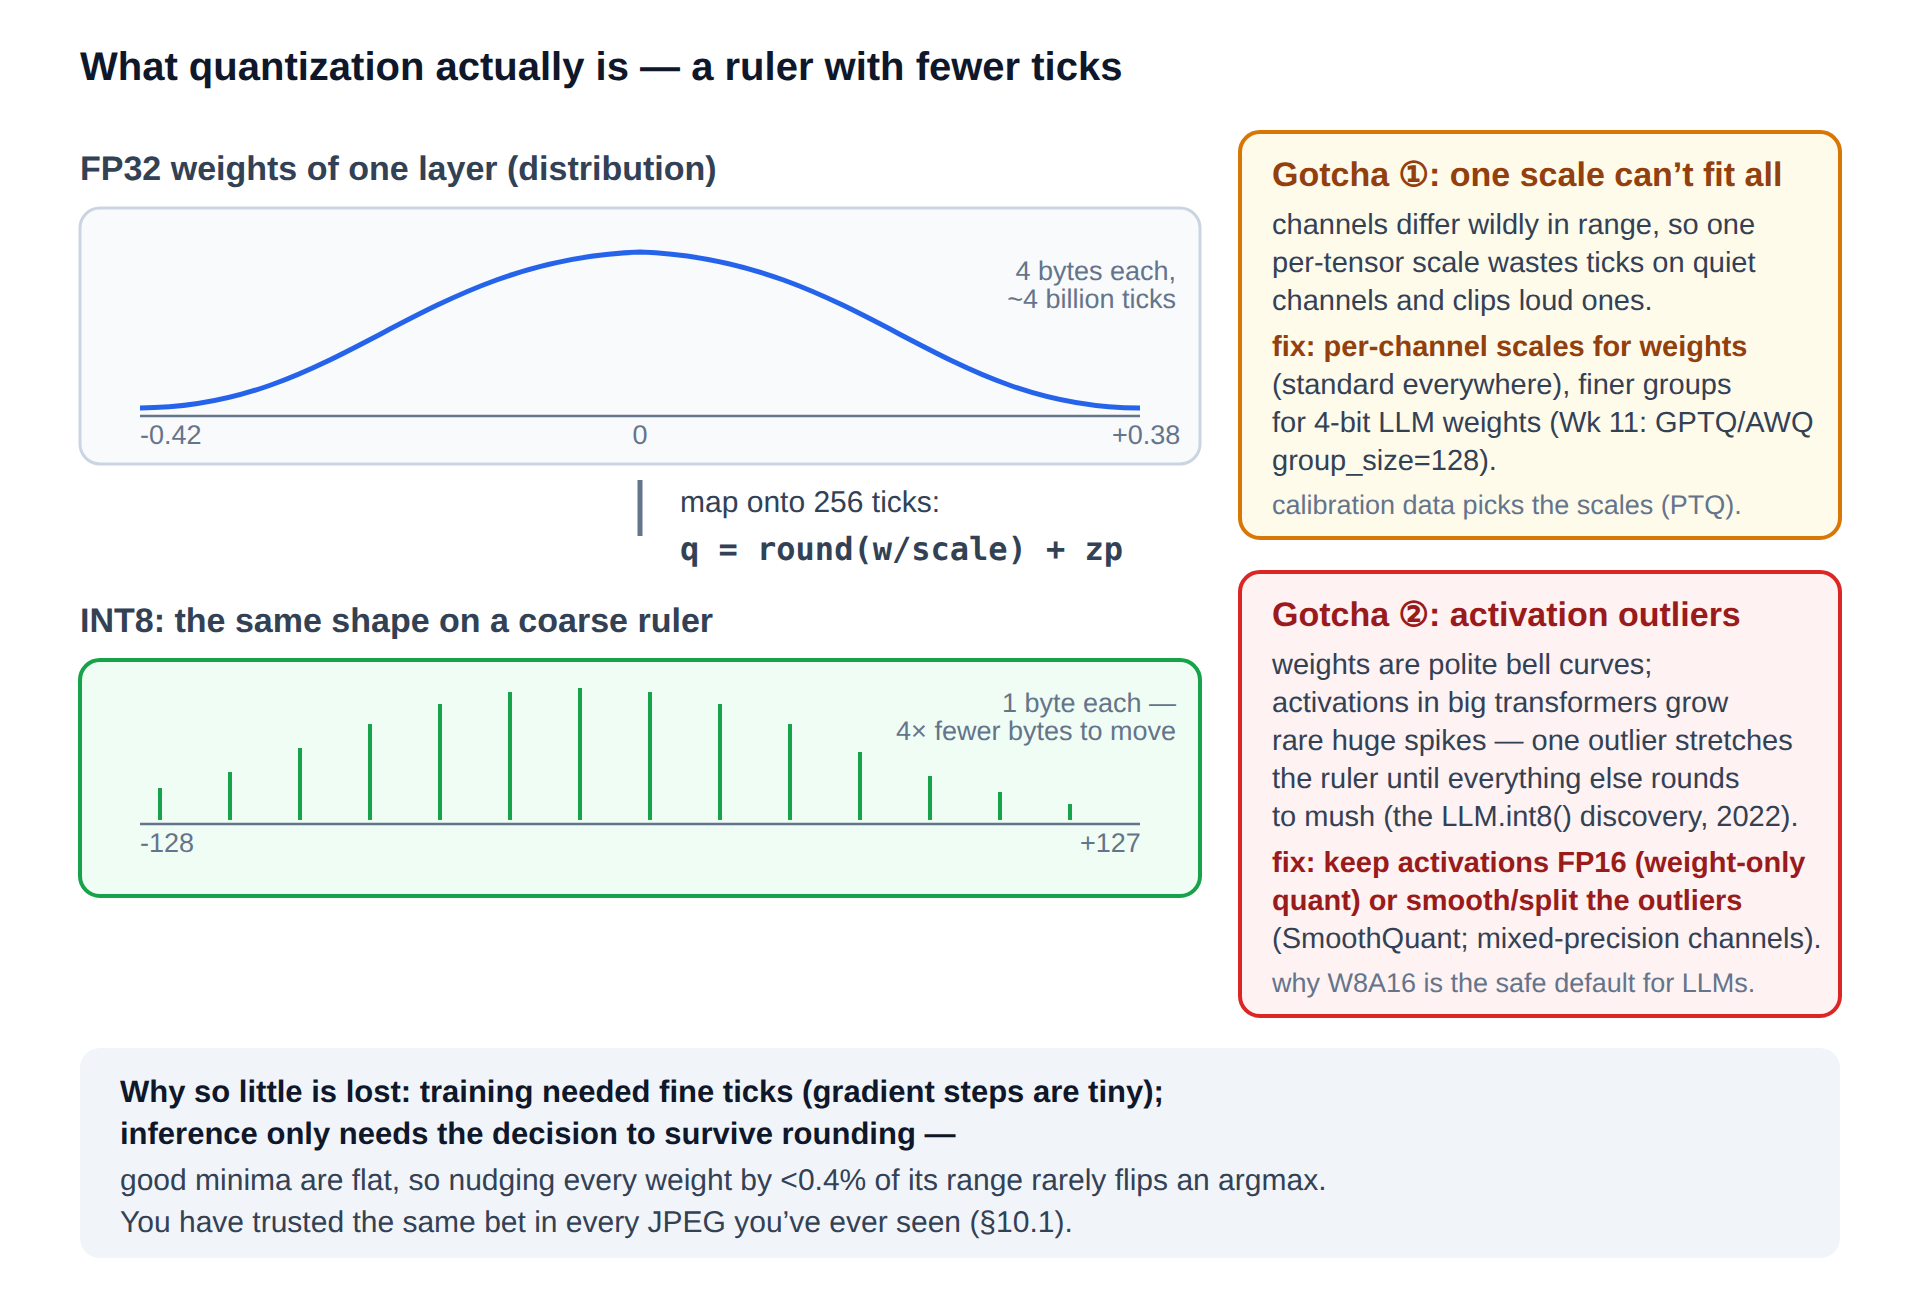
\includegraphics{figures/fig10-3_quantmap.png}}\\[3pt]
  \figcaption{그림 10-3  양자화는 텐서가 실제로 사용하는 범위 위에 더 거친 자를 놓는 작업이다. 기술의 핵심은 눈금을 배치하는 방식(스케일, 채널별)에 있다. 주의할 점은 채널마다 범위가 다르고 트랜스포머 활성값에 이상치가 숨어 있다는 것이다.}
\end{tbbfigure}

\subsection*{자 자체의 차이: 부동소수점은 관대하고 정수는 그렇지 않은 이유}

눈금을 놓기 전에 눈금의 재료부터 살펴보자. 이 절의 어려움은 하나의 구조적 차이에서 비롯된다. \textbf{부동소수점 수는 자기만의 자를 지닌다.} 지수 비트가 각 값의 스케일을 개별적으로 정하므로 0.001 근처의 수와 1,000 근처의 수가 모두 가수부의 전체 해상도를 얻는다. 지난 5주간 실습하면서 범위를 한 번도 고민하지 않아도 되었던 이유다. \textbf{정수에는 지수가 없다.} 하나의 고정된 자 위에 놓인 위치일 뿐이므로, \textit{다른 누군가}가 텐서 전체에 적용할 자의 범위를 한 번 정해야 한다. 그 누군가가 바로 보정이다. 아래에서 볼 모든 함정, 즉 서로 다른 채널과 범위를 늘리는 이상치(outlier)는 많은 값이 하나의 스케일을 함께 써야 한다는 데서 생긴다. 부동소수점은 관대하지만, 정수는 그 관대함을 사용자에게 위임한다.

부동소수점 계열은 30초쯤 들여 살펴볼 가치가 있다. 이제 모든 GPU 사양표에 등장하기 때문이다. \textbf{FP32} (부호 1비트 · 지수 8비트 · 가수 23비트)는 기준이 되는 자다. \textbf{FP16} (1·5·10)은 바이트를 절반으로 줄이는 대신 \textit{범위}도 줄여 최댓값이 65,504다. FP16 학습에서 작은 경사가 0으로 사라지지 않게 손실 스케일링 기법이 필요한 이유다. \textbf{BF16} (1·8·7)은 반대의 절충을 택한다. FP32의 지수 범위를 그대로 유지하고 거친 가수부(십진수 약 3자리)를 대가로 치른다. 경사가 오버플로하지 않아 학습에서 각광받지만, \textit{서빙}에서는 FP16보다 이득인 경우가 드물다. 둘 다 2바이트이고 대부분의 GPU에서 속도도 같다. \textbf{FP8}은 Hopper/Ada 하드웨어에서 지원한다. H100과 플릿의 L4에도 관련 회로가 있다. E4M3 (±448, 가중치와 활성값용)와 E5M2 (±57,344, 경사용)의 두 형식이 있으며, \textit{정수 수준의 저장 비용에 약간의 자체 스케일링을 남긴 형식}으로 이해하면 좋다. 실제로는 여전히 보정하지만 INT8보다 불완전한 스케일을 훨씬 잘 견딘다. \textbf{INT8/INT4}는 이 장에서 다루는 맨몸의 자다. 가장 저렴하고 빠르지만 아래에서 설명할 눈금 배치 기술에 전적으로 의존한다.

반복되는 혼란을 막아 줄 구현상의 각주가 하나 있다. INT8 계층 안에서 INT8 × INT8의 곱은 \textbf{INT32에 누적}된다. 수천 개 항을 오버플로 없이 더한 뒤, 결과가 나갈 때 출력 스케일로 \textit{재양자화}한다. 따라서 양자화 모델의 정확도 문제는 사실상 "누산기가 오버플로했다"는 데서 생기지 않는다. 언제나 "이 텐서에 맞지 않게 눈금을 배치했다"는 문제다. 이에 맞게 진단해야 한다. 해결책은 연산 폭이 아니라 스케일과 보정(calibration)에 있다.

\subsection*{눈금 배치하기: 스케일, 세분성, 보정}

실제 수치로 작동 원리를 한 번 살펴보자. 네 줄이면 충분하며 이후의 모든 약어에서 신비를 걷어 낼 수 있다. 가중치 범위가 [−0.42, +0.38]인 계층을 생각하자. 대칭 INT8은 −127…+127의 눈금을 사용하므로 \textbf{scale = max|w| ÷ 127 = 0.42 ÷ 127 ≈ 0.00331}이고 zero\_point = 0이다. 가중치 0.087231은 q = round(0.087231 ÷ 0.00331) = \textbf{26}이 되어 1바이트에 저장된다. 연산할 때 역양자화하면 26 × 0.00331 = 0.08606이다. 모두가 논하는 "손실"이란 약 0.0012, 즉 눈금 하나의 3분의 1에 해당하는 이 반올림 오차가 전부다. 이는 네트워크가 이미 견디는 잡음 하한 \textit{아래}에 있다. §10.1에서 본 평평한 최솟값 논증을 수치로 확인한 셈이다. 25 MB짜리 FP32 계층 전체는 \textasciitilde{}6.3 MB와 몇 개의 부동소수점 스케일로 바뀐다. 양자화란 \textit{그게 전부}다. 이 절의 나머지 내용인 세분성, 보정, 이상치, 게이트는 이 네 줄짜리 이야기가 어긋나는 경우를 다룬다.

앞의 예에서는 가중치가 0을 중심으로 양쪽에 걸쳐 있어 \textit{대칭} 자(zero\_point = 0)를 사용했다. 활성값은 그렇지 않은 경우가 많다. ReLU를 지난 계층의 출력 범위가 \textbf{[0, 6.2]}라면 대칭 자는 256개 눈금의 절반을 절대 나타나지 않는 음수에 낭비한다. 그 결과 아무 이유 없이 간격이 두 배가 된다(6.2 ÷ 127 = 0.049). \textbf{zero\_point}는 바로 이 문제를 해결한다. \textit{비대칭} 자는 scale = 6.2 ÷ 255 = 0.024, zero\_point = −128로 설정해 실수 0.0을 코드 −128에 대응시킨다. 이제 256개 눈금 모두가 실제 값의 범위를 덮고, 간격은 절반이 된다. q = round(w/scale) + zero\_point의 알쏭달쏭한 두 번째 매개변수는 자를 옮겨 어느 부분도 낭비하지 않게 하는 역할을 한다.

양자화의 모든 기술은 눈금 배치로 귀결된다. \textbf{텐서마다 하나의 스케일}을 쓰는 방식이 가장 둔감하며, 계산해 보면 그 정도가 드러난다. 채널 7의 가중치 범위는 ±2.0이고 채널 300은 ±0.05라고 하자. 공유 스케일은 채널 7을 수용해야 하므로 scale = 2.0 ÷ 127 ≈ 0.0157이다. 그러면 채널 300의 \textit{전체 범위}가 약 세 눈금 안에 갇힌다. 전형적인 가중치 0.02는 q = round(0.02 ÷ 0.0157) = 1로 양자화되고 0.0157로 역양자화된다. 모든 가중치에서 체계적으로 \textbf{21\% 오차}가 난다. 채널 300에 자체 자(scale = 0.05 ÷ 127 ≈ 0.00039)를 주면 같은 가중치가 q = 51 → 0.0201이 되어 \textbf{0.4\% 오차}에 그친다. 채널마다 부동소수점 하나만 더 저장하면 오차를 50분의 1로 줄일 수 있다. 그래서 \textbf{채널별 스케일}, 즉 출력 채널마다 하나의 자를 두는 방식이 가중치의 보편적인 표준이다. 4비트 LLM 양자화는 \textbf{그룹별 스케일}로 더 세분화한다. 가중치 128개마다 하나를 두는 방식이며, 11주 차의 GPTQ/AWQ 용어를 여기서 미리 만난다. 범위는 어디서 구할까? 가중치는 알려진 상수이므로 파일에서 읽으면 된다. \textit{활성값}은 누군가 관찰해야 한다. \textbf{보정}은 대표 입력 수백 개를 모델에 통과시키고 계층마다 활성값 범위를 기록해 그에 맞는 스케일을 고른다. 이것이 \textbf{학습 후 양자화(PTQ)}다. 재학습이 필요 없고 CI에서 몇 분이면 끝난다. 품질은 보정 세트의 품질과 정확히 같다. 이미지 모델을 낮 사진만으로 보정하면 밤 입력은 클리핑된다. 대안인 \textbf{양자화 인식 학습(QAT)}은 미세 조정 중 반올림을 모사해 네트워크가 그 영향을 피해 학습하게 한다. PTQ가 잃은 정확도를 되찾지만 학습 파이프라인만큼 비용이 든다. 이 책은 PTQ를 사용하지만, 언제 그 너머의 방법이 필요한지는 알아야 한다. 그림 10-4를 참고하자.

보정은 관찰한 활성값 더미를 어떻게 하나의 스케일로 바꿀까? 정교함이 높아지는 순서로 세 가지 방법이 있으며, 그 차이는 결코 이론에 그치지 않는다. \textbf{최솟값–최댓값}은 실제 극값을 택한다. 정직하지만 취약하다. 활성값 999개가 6.0 아래에 있는데 하나의 특이한 값만 41.0에 이르면 스케일은 41 ÷ 127 ≈ 0.32가 된다. 실제 값 전체가 사용 가능한 127개 중 약 \textbf{열아홉 눈금}(6 ÷ 0.32)에 몰린다. 이상한 입력 하나가 영구적으로 해상도 3비트를 앗아 간 셈이다. \textbf{백분위수} 방식은 예컨대 99.99번째 백분위수를 기준으로 이상치를 클리핑한다. scale = 6.3 ÷ 127 ≈ 0.05가 되어 일반 값은 자 전체를 되찾고, 드문 41.0은 맨 위 눈금에서 포화된다. 드문 값에 유한한 오차를 허용하는 대신 나머지 모든 값의 해상도를 얻는다. 거의 언제나 올바른 절충이다. \textbf{엔트로피/KL 보정}은 TensorRT의 기본값이며 이 절충을 자동화한다. 후보 클리핑 임곗값을 훑어 FP32 분포와 그 INT8 그림자 사이의 정보 손실이 가장 작은 값을 고른다. 어떤 방식을 택하든 계층 관계를 기억해야 한다. \textit{방법}은 보정 세트가 만든 세계 안에서 자를 조절하지만, 그 세계 자체를 정의하는 것은 \textit{세트}다. 앞의 낮/밤 실패가 어떤 방법 선택보다 중요한 이유다.

두 번째 함정은 현대 LLM 스택의 형태를 좌우했으므로 따로 살펴볼 가치가 있다. 가중치는 얌전한 종 모양 분포를 보이지만, \textbf{대형 트랜스포머의 활성값은 그렇지 않다.} 일부 채널에서 전형적인 크기의 \textasciitilde{}100×에 이르는 드물고 거대한 스파이크가 나타난다. 2022년 LLM.int8() 연구로 널리 알려진 현상이다. 이상치 하나가 자를 늘려 정상 값을 모두 뭉개진 값으로 반올림하게 만든다. 활성값을 단순하게 양자화하면 13B 모델의 퍼플렉시티가 폭발한다. 실용적인 대응책은 앞으로 만날 순서대로 다음과 같다. \textbf{가중치 전용 양자화(weight-only quantization)}는 가중치를 INT8/INT4로 저장하되 FP16으로 연산한다. §10.2에서 바이트를 지배하는 것이 가중치임을 확인했으므로 대부분의 이점이 남으며, LLM의 기본 방식이다. \textbf{평활화}는 SmoothQuant 방식의 재스케일링으로 활성값의 범위 부담을 가중치 쪽으로 옮긴 뒤 둘 다 양자화한다. \textbf{혼합 정밀도(mixed precision)}는 이상치 채널만 FP16으로 유지한다. 이번 주 CNN급 실습 모델의 활성값은 온순하므로 전체 W8A8 INT8이 잘 동작한다. 이상치 이야기는 11주 차에 다시 꺼낼 수 있게 기억해 두자.

\begin{tbbfigure}
  \adjustbox{max width=0.94\linewidth,max totalheight=0.46\textheight}{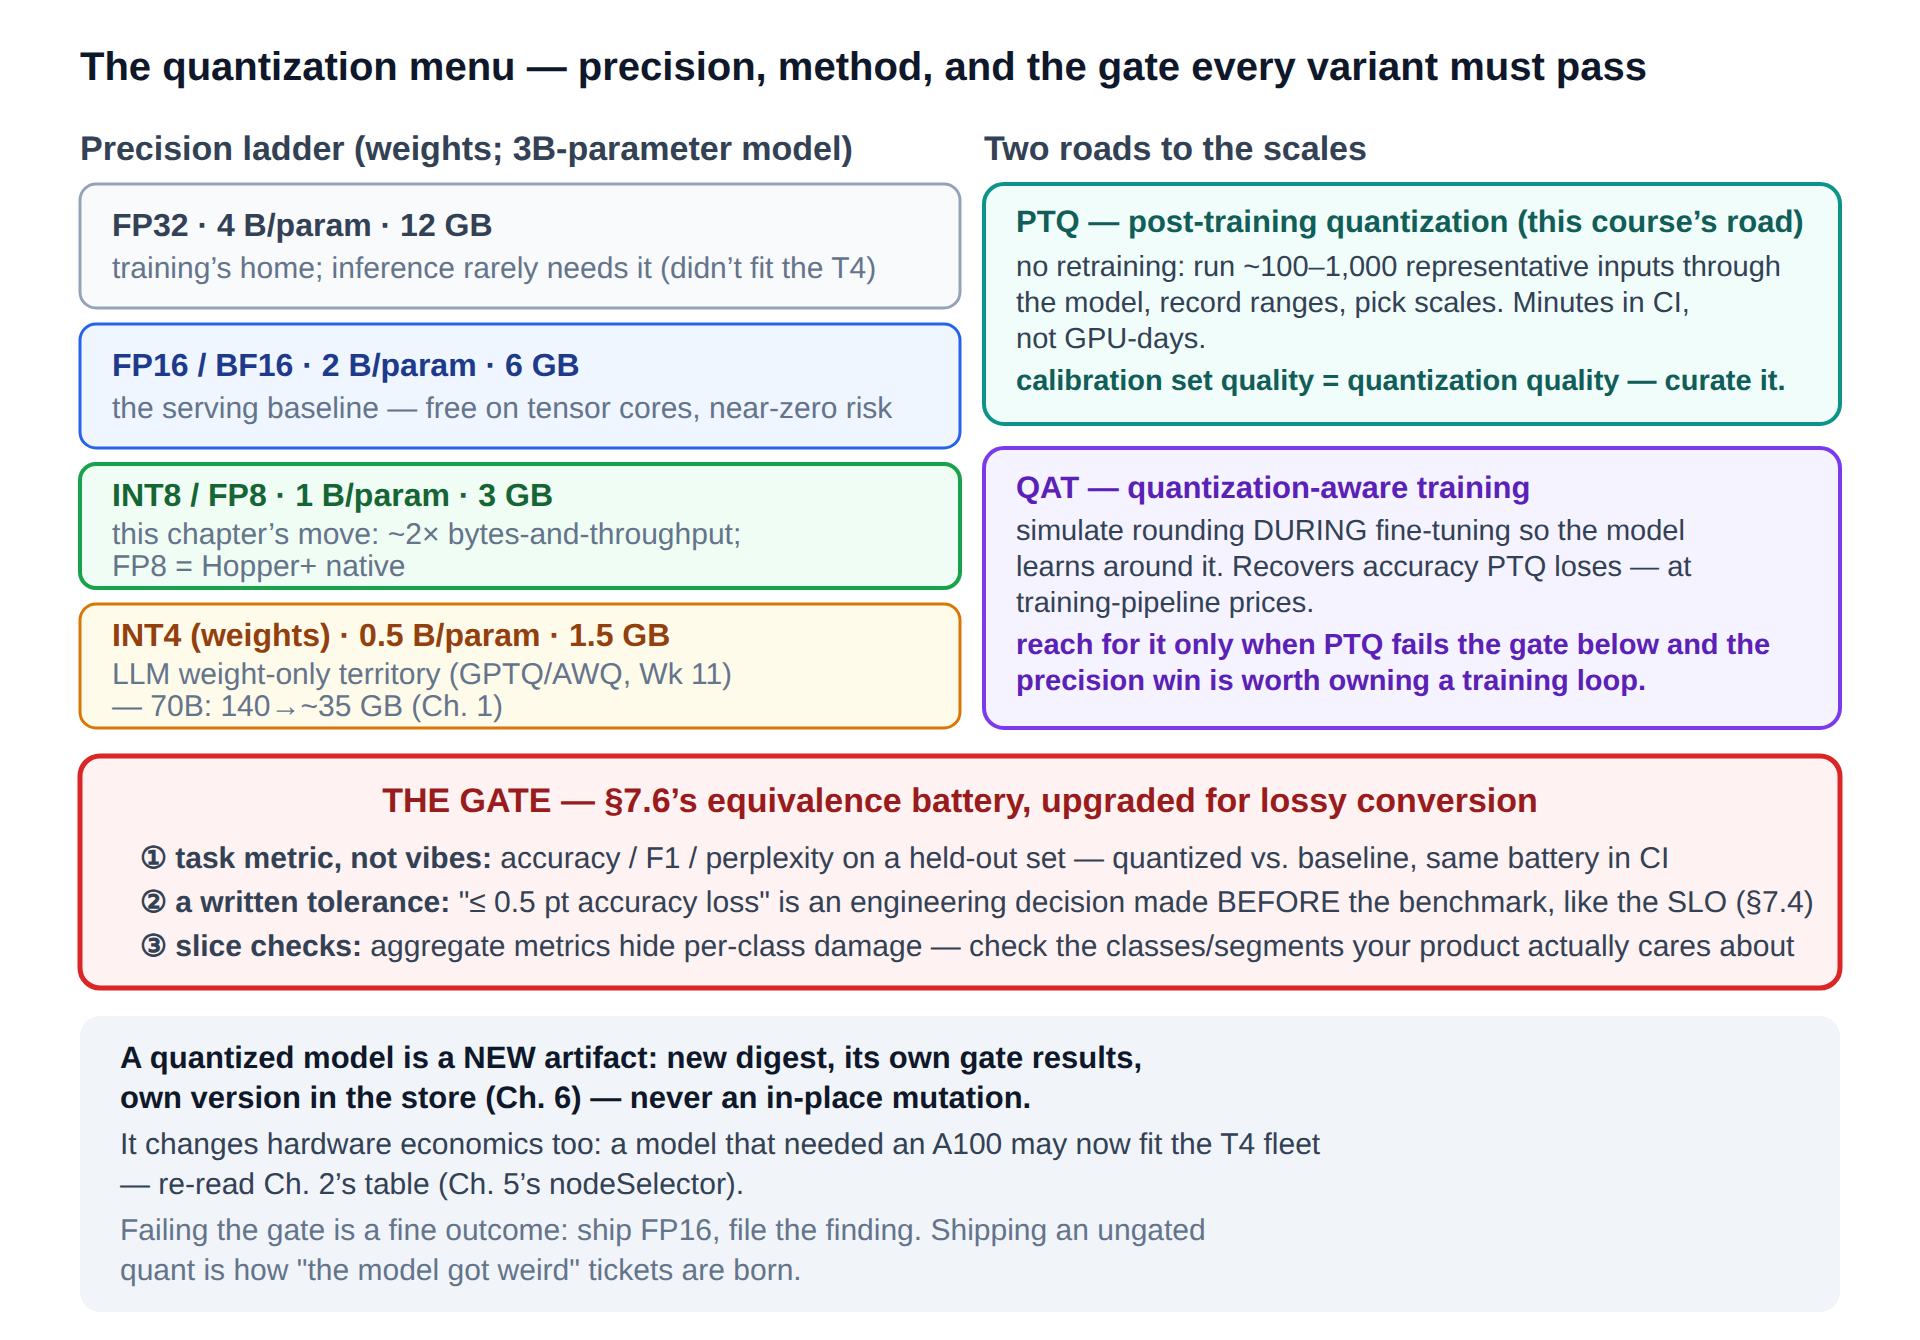
\includegraphics{figures/fig10-4_quantmenu.png}}\\[3pt]
  \figcaption{그림 10-4  선택지와 게이트. 정밀도의 단계(제1장의 70B 모델은 INT4에서 140 GB → \textasciitilde{}35 GB), PTQ 대 QAT, 그리고 모든 손실 산출물이 버전을 얻기 전에 통과해야 할 게이트를 보여 준다.}
\end{tbbfigure}

\subsection*{게이트: 손실 산출물이 배포 자격을 얻는 법}

사례 10-A의 E행을 엔지니어링이라 부를 수 있는 것은 처리량을 보기 전에 \textbf{게이트}를 거쳤기 때문이다. 양자화 모델은 \textit{변경된} 모델이다. 본질적으로 무손실인 변환을 위해 만든 §7.6의 동등성 검사를 손실 변환에 맞게 강화해야 한다. 게이트는 세 부분으로 구성된다. 첫째, \textbf{감이 아니라 작업 지표}를 사용한다. 별도 보관 세트에서 정확도, F1 또는 퍼플렉시티를 기준 모델과 양자화 모델 사이에 비교한다. 들뜬 사람이 임의로 실행하는 것이 아니라 CI가 실행한다. 둘째, \textbf{허용 오차를 문서로 명시}한다. "≤ 0.5 points top-1 loss"는 벤치마크 \textit{전에} 내리는 엔지니어링 결정이다. 정확도에 대응하는 SLO이며, SLO와 마찬가지로 논쟁을 계산으로 바꾼다. 셋째, \textbf{슬라이스를 점검}한다. 집계값은 특정 구간에 집중된 손상을 감춘다. 전체적으로 0.2포인트 하락했지만 제품의 존재 이유인 클래스 하나에서는 4포인트가 무너질 수 있다. 따라서 게이트는 이해관계자가 중요하게 여기는 슬라이스를 검사한다. 터미널 기록 10-3은 통과한 실행을 보여 준다.

\begin{terminalbox}
\begin{Verbatim}[breaklines=true,breakanywhere=true,fontsize=\small,formatcom=\color{tbbtermfg},codes=\tbbcodeactive]
$ python gate.py --baseline clf_fp16 --candidate clf_int8 --tol 0.5
held-out set: 10,000 images (never seen by calibration)
  baseline   top-1  76.14%
  candidate  top-1  75.92%     delta -0.22 pt   (tol 0.5)  PASS
  worst slice: "streetcar" -1.8 pt  (slice fail-line 3.0)  flag
  logit drift |p99|: 0.041
verdict: PROMOTE -> s3://models/clf/v8-int8/  (new digest)
# fail path exists and is honorable: ship FP16, file the finding.
# an ungated quant is how "the model got weird" tickets are born.
\end{Verbatim}
\end{terminalbox}
\figcaption{터미널 기록 10-3  게이트 통과. 허용 오차는 실행 전에 명시했고, 슬라이스 검사는 집계값이 손상을 감추는 곳을 살폈다. 출력은 자체 다이제스트를 지닌 새 산출물이다. 기존 산출물을 제자리에서 변경하지 않는다.}

두 가지 운영상의 귀결로 이 절을 마무리하자. \textbf{양자화 모델은 새로운 산출물}이다. 새 다이제스트를 갖고, 자체 게이트 보고서를 옆에 저장하며, 모델 스토어(제6장)에 별도 버전으로 둔다. 저장소가 여러 버전을 나란히 두도록 설계된 이유(제9장의 기관 ④)가 바로 이런 롤백에 있다. 또한 \textbf{양자화는 하드웨어의 가격표를 다시 쓴다.} A100의 VRAM이 필요하던 모델이 이제 T4 플릿에 들어갈 수 있다. 제1장의 대표 사례였던 70B 모델은 INT4에서 140 GB에서 \textasciitilde{}35 GB로 줄어 저렴한 GPU 네 장이나 큰 GPU 한 장이면 된다. 정밀도를 바꿀 때마다 제2장의 플릿 표를 다시 읽어야 한다. 제5장의 \code{nodeSelector} 질문인 "어느 GPU 레이블을 겨냥할 것인가?"에는 새로운 정답이 생기며, 구속 차원이 달라졌을 수도 있다.

\begin{calloutbox}{tbbpurple}{tbbpurplefill}
{\normalsize\bfseries\color{tbbpurple}생각해 보기}\par\vspace{3pt}
\begin{tbbitemize}
  \item 보정 세트는 지난달 트래픽에서 표본으로 뽑은 이미지 500장이다. 다음 주에 새로운 국가에서 제품을 출시한다. PTQ가 겪도록 설정된 실패 유형과 이에 해당하는 §10.3의 조절점(눈금 배치)을 설명하고, 저렴하게 완화할 방법을 제시하라.
  \item 자신의 프로젝트 모델에 적용할 게이트 문장을 작성하라. 지표, 별도 보관 세트, 허용 오차, 반드시 점검할 슬라이스 하나를 포함해야 한다. 이어서 회의적인 팀원에게 그 허용 오차 수치의 출처를 설명하고 정당화하라.
  \item 가중치 전용 INT4는 활성값을 FP16으로 유지하므로 연산 자체는 변하지 않는다. 그런데도 배치 1 LLM의 지연 시간은 거의 4× 개선된다. 이를 §10.2와 모순 없이 두 문장으로 설명하라. 어느 하한이 움직였는가?
  \item 어떤 공급업체가 "정확도 손실 0을 보장하는 INT8이며 보정도 필요 없다"고 주장한다. 이 절을 바탕으로 그 주장의 실제 의미를 드러낼 세 가지 질문을 제시하라.
  \item BF16은 FP32의 지수를 유지하면서 가수부 16비트를 버리고, FP16은 가수부를 더 많이 유지하면서 범위를 버린다. "자 자체의 차이" 소절을 바탕으로 BF16이 학습에서 각광받은 이유와 서빙에서는 둘 중 어느 것도 상대보다 우위가 아닌 이유를 설명하라. FP8-E4M3이 INT8에는 없는 무엇을 제공하는지도 덧붙여라.
\end{tbbitemize}
\end{calloutbox}

\section{그래프 컴파일: 더 적은 왕복과 실행}

양자화가 바이트를 줄였다면 컴파일은 \textit{낭비}를 공격한다. 그 낭비를 보려면 즉시 실행이 정직하고 순진하게 일하는 모습을 관찰하면 된다. 즉시 실행 PyTorch는 Python이 모델을 만나는 순서대로 실행한다. 각 연산이 자체 GPU 커널을 실행하고, VRAM에서 입력을 읽은 뒤 출력을 다시 기록한다. conv → batch-norm → ReLU → add 연쇄에서는 커널을 네 번 실행한다. 각 실행은 고정 비용으로 제9장의 \textbf{a} 일부를 차지한다. 메모리 병목 환경에서는 더 나쁜 일도 생긴다. \textbf{중간 활성값이 VRAM을 세 번 왕복}한다. §10.2에서 비용으로 보아야 한다고 배운 바로 그 바이트를 몇 마이크로초만 존재하는 값에 쓴다. 즉시 실행의 유연성은 어떤 Python과 제어 흐름도 허용하므로 프로토타입에 적합하다. 이 절은 더는 쓰지 않는 유연성에 비용을 내지 않을 때 어떤 일이 생기는지를 다룬다.

\begin{tbbfigure}
  \adjustbox{max width=0.94\linewidth,max totalheight=0.46\textheight}{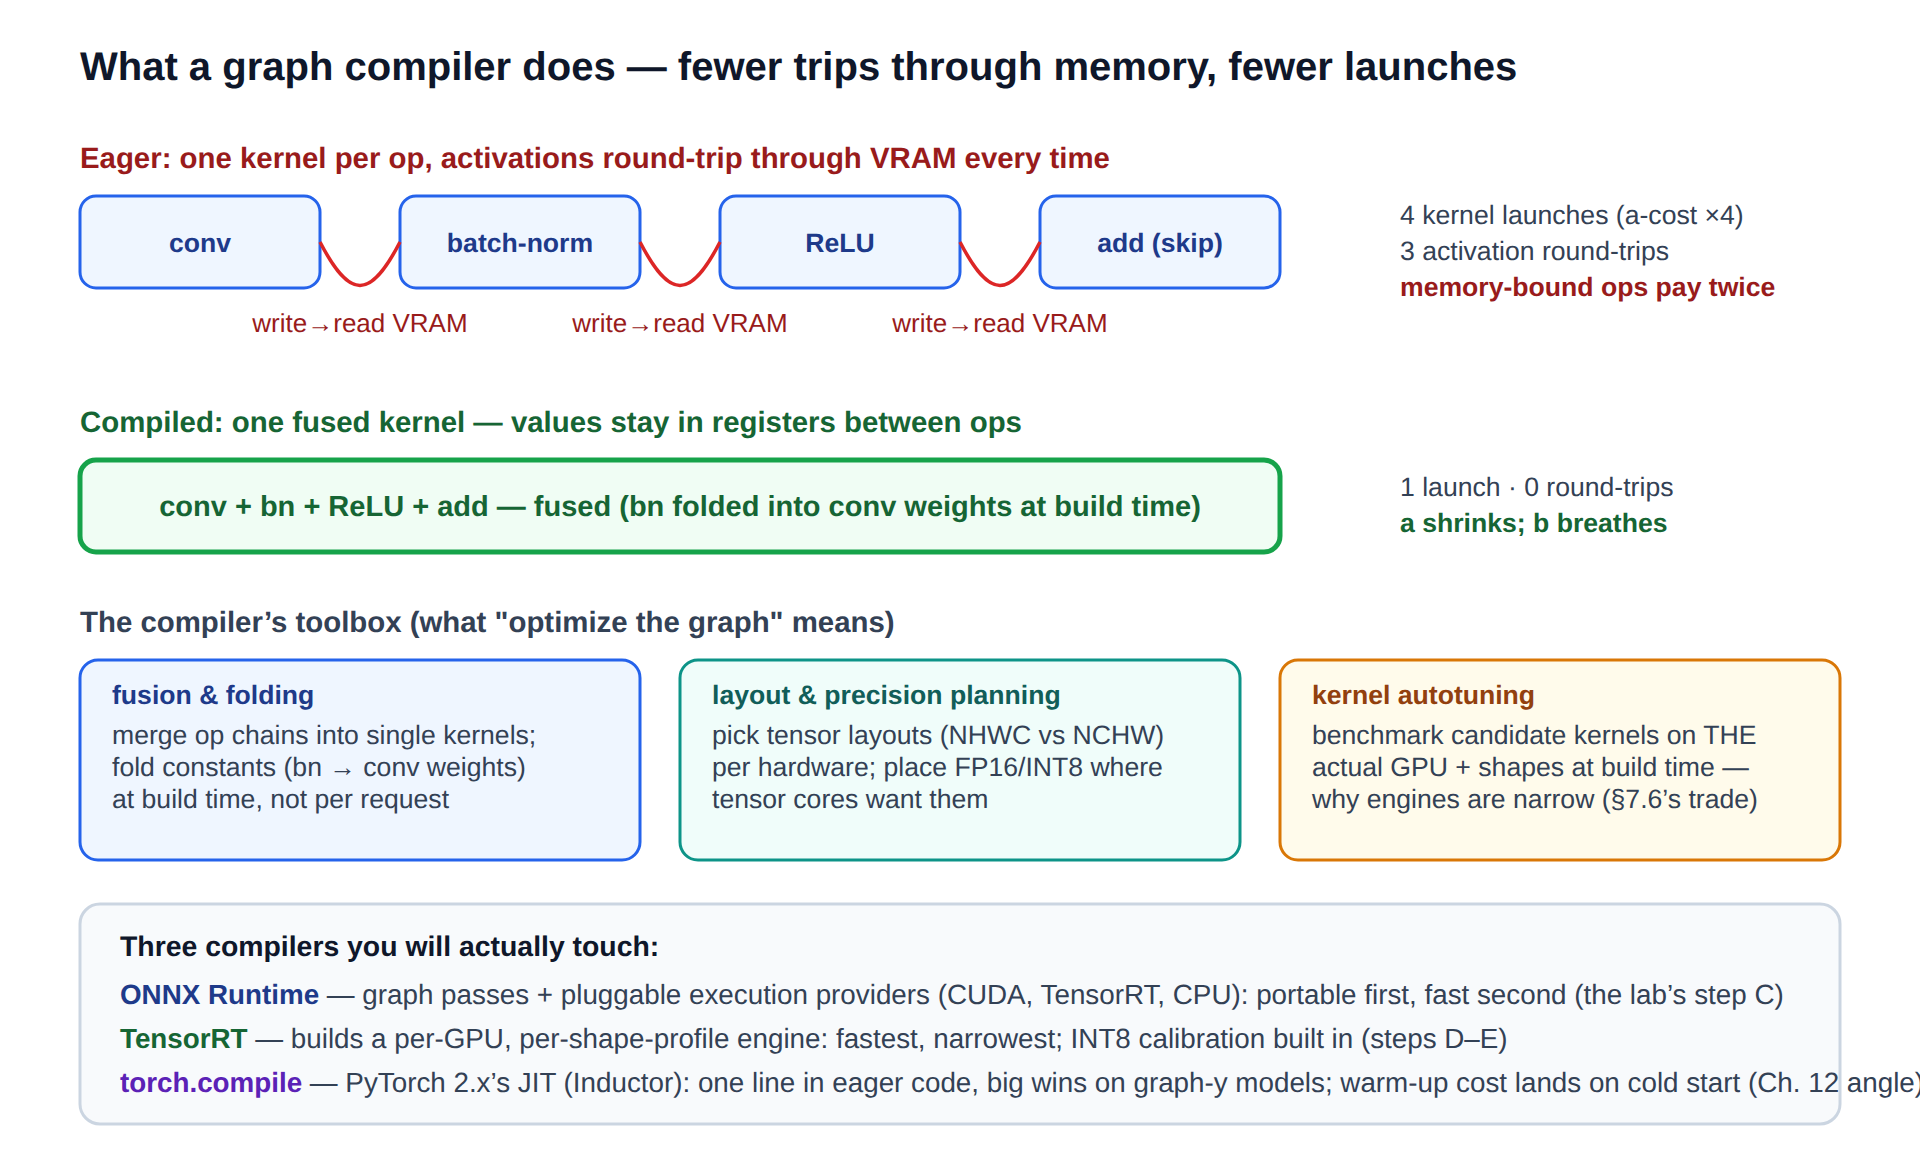
\includegraphics{figures/fig10-5_compiler.png}}\\[3pt]
  \figcaption{그림 10-5  컴파일러의 역할. 즉시 실행에서는 연산마다 커널 하나가 실행되고 활성값이 메모리를 왕복한다. 컴파일하면 커널이 융합되고 값이 레지스터에 머문다. a가 줄고, 메모리 벽을 세 번이 아니라 한 번만 건넌다.}
\end{tbbfigure}

\subsection*{도구 상자: "그래프 최적화"의 실제 의미}

컴파일러에 전체 그래프, 즉 §7.6의 내보낸 산출물을 건네면 네 계열의 재작성이 가능해진다. 내보내기 형식이 존재하는 이유다. \textbf{융합}은 원소별 연산과 정규화 연산의 연쇄를 값을 생성하는 커널에 합친다. conv+bn+ReLU+add가 \textit{한 번}의 실행이 되고 중간값은 레지스터를 떠나지 않는다. 네 번 실행하고 세 번 왕복하는 대신 벽을 한 번만 건넌다. \textbf{상수 폴딩(constant folding)}은 빌드 시점에 계산할 수 있는 것을 미리 계산한다. 학습이 끝나면 상수일 뿐인 batch-norm의 스케일과 이동값을 conv의 가중치에 합치고, reshape를 접으며, 실행되지 않는 분기를 없앤다. \textbf{레이아웃과 정밀도 계획}은 텐서 코어가 요구하는 특정 메모리 레이아웃(NHWC 대 NCHW)과 위치별 정밀도를 맞춘다. 연산마다 전치하지 않고 컴파일러가 전체 텐서를 한 번에 다시 배치한다. \textbf{커널 오토튜닝(autotuning)}은 각 융합 연산에 존재하는 수십 가지 후보 구현(타일링, 루프 펼치기, 텐서 코어 경로)을 평가한다. 빌드 시점에 \textit{실제 GPU와 실제 형상에서 벤치마크}하고 가장 좋은 구현을 결과물에 넣는다. 마지막 항목은 단일 기법으로 가장 큰 개선을 내는 동시에 §7.6에서 이미 본 절충의 원인이 된다. \textbf{출력은 하나의 GPU 모델과 하나의 형상 범위에 결합된다.} 가장 빠르지만 가장 좁다.

\subsection*{직접 계산하기: 8.4 → 3.1 ms는 어디에서 사라졌는가}

"컴파일러가 a를 줄였다"는 말을 냅킨 한 장에서 계산할 수 있다면 구호로 남겨 둘 이유가 없다. ResNet급 분류기는 즉시 실행 순방향 패스마다 약 \textbf{175개의 CUDA 연산}을 수행한다. conv 약 53개와 각각의 batch-norm, \textasciitilde{}49개 ReLU, 16개 잔차 덧셈, 풀링과 헤드가 포함된다. 즉시 실행에서는 각 연산이 Python 디스패치와 커널 실행 비용을 낸다. 이를 \textbf{연산당 \textasciitilde{}25 μs의 오버헤드}라고 하면 한 패스에 175 × 25 μs ≈ \textbf{4.4 ms의 순수 관리 비용}이 붙는다. GPU가 실제 작업으로는 전혀 보지 못하는 시간이다. TensorRT는 이 175개 연산을 \textbf{\textasciitilde{}60개 커널}로 융합하고 연산마다 Python을 거치지 않은 채 C++에서 실행한다. 오버헤드는 \textasciitilde{}0.3 ms로 줄어든다. 메모리 벽의 몫도 더해 보자. 배치 1의 중간 활성값은 총 \textasciitilde{}45 MB이고, 즉시 실행의 개별 bn/ReLU/add 커널이 이를 다시 읽고 쓰면서 320 GB/s에서 \textbf{피할 수 있는 트래픽 90 MB ≈ 0.3 ms}를 만든다. 관리 비용(≈4.1 ms 절감) + 왕복(≈0.3 ms) + 상수 폴딩으로 완전히 삭제한 수십 개 연산을 합치면 \textbf{a에서 사라진 5.3 ms}가 된다. 이 계산은 터미널 기록 10-6에서 확인할 수 있는 미묘한 현상도 예측한다. 배치 32에서는 활성값이 32× 커져 피할 수 있는 트래픽이 \textasciitilde{}3 GB, 즉 패스당 ≈ 9 ms이고 \textit{항목당} \textasciitilde{}0.3 ms가 된다. 따라서 융합은 b도 조금씩 줄인다. C에서 D로 갈 때 적합 결과의 b가 1.74 → 1.62 ms로 소폭 내려가는 이유다.

상수 폴딩의 묘기도 온전히 살펴보자. 세 줄의 대수만으로 네트워크에서 연산자 계열 하나를 통째로 삭제한다. 추론 시 batch-norm은 conv 출력 z = Wx + b에 y = γ·(z − μ)/σ + β를 적용한다. 학습이 끝나면 네 매개변수는 모두 \textbf{고정된 상수}다. 대입하고 항을 다시 묶으면 \textbf{y = (γ/σ)·W·x + (γ(b − μ)/σ + β)}가 된다. 이는 가중치 W′ = (γ/σ)W, 편향 b′ = γ(b − μ)/σ + β인 또 다른 합성곱일 뿐이며 \textit{빌드 시점}에 계산할 수 있다. 융합을 시작하기도 전에 53개의 batch-norm이 0개가 된다. 이는 §7.6의 동등성 검사에도 조용한 경고를 보낸다. 폴딩한 네트워크는 대수적으로 같지만 부동소수점 연산의 \textit{결합 순서가 달라진다}. 컴파일러가 손대는 순간 비트 단위 동일성은 사라진다. 그래서 검사는 비트가 아니라 허용 오차를 확인한다.

\subsection*{세 가지 컴파일러, 하나의 결정 패턴}

\textbf{ONNX Runtime}은 이식성 있는 중간 지점이다. 그래프 패스(융합, 폴딩)를 적용한 뒤 CUDA, TensorRT, CPU 등의 플러그형 \textbf{실행 공급자}에 디스패치한다. 하나의 산출물을 어디서나 최고는 아니지만 준수한 속도로 서빙할 수 있다. 사례 10-A의 C행에서 별다른 대가 없이 1.4×를 얻었으며, 이기종 플릿에서 합리적인 기본값이다. \textbf{TensorRT}는 NVIDIA에 모든 것을 건다. \textit{빌더}가 그래프와 \textbf{최적화 프로파일}, 즉 전송을 약속한 형상 범위인 min/opt/max 배치와 차원을 받아 정확한 GPU에 맞춰 계층별 커널을 오토튜닝한다. 선택적으로 INT8도 보정하며, §10.3의 스케일을 같은 빌더가 계산한다. 그 결과 빠르게 로드되고 가장 빠르게 실행되는 직렬화된 계획인 \textbf{엔진}이 나온다(D–E행). 엔진의 좁은 범위는 이론이 아니라 운영 현실이다. 프로파일 밖의 형상을 거부하고 다른 GPU 세대에서는 실행되지 않는다. 실습에서 산출물 이름을 \code{t4/\allowbreak clf\_int8.plan}으로 지정하는 이유다. 제4장의 다이제스트 규율에 하드웨어 좌표가 추가되었다. \textbf{torch.compile} (PyTorch 2.x)은 즉시 실행에 자연스러운 경로다. 데코레이터 하나가 일반 Python에서 그래프를 캡처해 JIT 컴파일한다(Inductor). 워크플로를 거의 바꾸지 않고 그래프 중심 모델에서 큰 개선을 얻는다. 다만 비용이 다른 위치에 발생한다. 컴파일이 \textit{런타임}에 일어나므로 첫 요청이 워밍업 비용을 부담하고 준비 상태 프로브와 콜드 스타트 예산이 이를 흡수해야 한다. 제5장과 제12장에서 이 문제를 다룬다. 동적 제어 흐름은 그래프를 여러 작은 컴파일로 쪼갤 수 있다.

\begin{terminalbox}
\begin{Verbatim}[breaklines=true,breakanywhere=true,fontsize=\small,formatcom=\color{tbbtermfg},codes=\tbbcodeactive]
# the lab's two builds, in full (CI steps - never at pod start):
$ trtexec --onnx=clf.onnx --saveEngine=t4/clf_fp16.plan --fp16 \
          --minShapes=input:1x3x224x224 \
          --optShapes=input:16x3x224x224 \
          --maxShapes=input:32x3x224x224    # the shape PROMISE
$ trtexec --onnx=clf.onnx --saveEngine=t4/clf_int8.plan --int8 \
          --calib=calib.cache               # §10.3, inside the builder
# engines are per-GPU, per-profile: the t4/ prefix is load-bearing.
# send a 64-batch to a max=32 engine -> refused. the narrowness is real.
\end{Verbatim}
\end{terminalbox}
\figcaption{터미널 기록 10-4  TensorRT 엔진 빌드. 최적화 프로파일은 형상에 대한 약속이고, INT8 보정은 빌더 안에서 실행된다. 엔진은 GPU 좌표 없이는 살아남지 못하므로 산출물 경로에도 이를 포함한다.}

\begin{tbbtablewrap}
  \begin{tabular}{@{}>{\raggedright\arraybackslash}m{\dimexpr 0.1862\tbltextwidth-2\tabcolsep\relax} >{\raggedright\arraybackslash}m{\dimexpr 0.2128\tbltextwidth-2\tabcolsep\relax} >{\raggedright\arraybackslash}m{\dimexpr 0.2021\tbltextwidth-2\tabcolsep\relax} >{\raggedright\arraybackslash}m{\dimexpr 0.1862\tbltextwidth-2\tabcolsep\relax} >{\raggedright\arraybackslash}m{\dimexpr 0.2128\tbltextwidth-2\tabcolsep\relax}@{}}
  \arrayrulecolor{tbbnavy}\specialrule{1pt}{0pt}{0pt}
  \rowcolor{tbbtablehead}{\centering \bfseries\color{tbbnavy}도구} & {\centering \bfseries\color{tbbnavy}컴파일 시점} & {\centering \bfseries\color{tbbnavy}산출물과 범위} & {\centering \bfseries\color{tbbnavy}사례 10-A의 개선} & {\centering \bfseries\color{tbbnavy}치러야 할 대가} \\
  \arrayrulecolor{tbbnavy}\specialrule{0.7pt}{0pt}{2pt}
  {\textbf{ONNX Runtime}} & {로드 시점(그래프 패스) + EP 디스패치} & {EP가 있으면 어디서나 실행되는 하나의 .onnx} & {1.4× (C행)} & {준수하지만 최고는 아닌 속도, 연산 지원 범위의 경계} \\
  \arrayrulecolor{tbbtableborder}\hline
  {\textbf{TensorRT}} & {CI의 빌드 시점(GPU-프로파일마다 수분)} & {하나의 GPU + 형상 프로파일(shape profile)에 결합된 엔진} & {1.6–2.0× (D–E행)} & {좁은 범위: GPU별 산출물, 형상 거부} \\
  \arrayrulecolor{tbbtableborder}\hline
  {\textbf{torch.compile}} & {첫 호출의 런타임(JIT)} & {산출물 없음 — 데코레이터 하나, 캐시는 최선 노력} & {(벤치마크하지 않음)} & {콜드 스타트 경로의 워밍업, 새 형상마다 재컴파일} \\
  \arrayrulecolor{tbbnavy}\specialrule{1pt}{2pt}{0pt}
  \end{tabular}\par
  \figcaption{표 10-2  세 가지 컴파일러 한눈에 보기. 어느 행을 고를지는 속도의 문제이기 전에 워크플로에 관한 결정이다.}
\end{tbbtablewrap}

\subsection*{torch.compile 시간 측정 — JIT 비용은 실제로 어디에 붙는가}

표 10-2의 셋째 행은 별도의 기록으로 살펴볼 가치가 있다. 공간이 아니라 \textit{시간}의 절충이기 때문이다. 비용을 \textit{어디서}가 아니라 \textit{언제} 치르는지가 달라진다. 게다가 한 줄이면 적용할 수 있어 팀원이 가장 먼저 손댈 도구다. 분류기를 관찰해 보자.

\begin{terminalbox}
\begin{Verbatim}[breaklines=true,breakanywhere=true,fontsize=\small,formatcom=\color{tbbtermfg},codes=\tbbcodeactive]
>>> model_c = torch.compile(model)        # one line. too easy?
>>> t(model_c, batch=1)   # first call: Dynamo traces, Inductor
call 1:   38,400 ms       # autotunes kernels... on the SERVING pod
>>> t(model_c, batch=1)
steady:        6.1 ms     # vs eager 10.5 -> a real 1.7x. BUT:
>>> t(model_c, batch=7)   # a shape it has not seen ->
call 1:    9,200 ms       # recompile. every novel shape, again.
# the win is real and the bill is real: ~40 s on the cold-start path
# (Ch. 5's probes + Ch. 12's scale-out both notice), and dynamic
# shapes -> recompiles (mark_dynamic / bucketing, §10.5, tames it).
\end{Verbatim}
\end{terminalbox}
\figcaption{터미널 기록 10-5  torch.compile은 런타임에 비용을 낸다. 정상 상태에서는 컴파일러다운 개선을 주지만 첫 호출과 처음 보는 모든 형상도 컴파일러만큼 비용을 청구한다. TensorRT처럼 CI가 아니라 파드의 준비 상태 구간에 정확히 38 s가 붙는다.}

운영 관점에서는 이렇게 읽을 수 있다. \textbf{TensorRT는 컴파일을 CI로 옮겼고, torch.compile은 파드 위로 옮겼다.} 어느 쪽도 틀리지 않다. 후자는 반복 개발 속도에서 압도적이며 Python 때문에 내보낼 수 없는 모델에도 유용하다. 다만 38초는 반드시 \textit{어딘가}에 자리 잡아야 한다. 합당한 장소는 세 곳이다. \textbf{준비 상태 프로브 워밍업}은 파드가 Ready를 보고하기 전에 대표 형상을 실행하며, 제5장의 프로브가 설계 목적을 정확히 수행한다. \textbf{영속 컴파일 캐시}는 이미지나 볼륨에 담아 배포한다. 캐시 키에 GPU, 버전, 형상이 포함되므로 최선 노력 방식이다. \textbf{사전 내보내기}는 \code{torch.export} + AOTInductor를 사용한다. 즉시 실행 모델에 CI에서 빌드한 산출물을 제공하려는 생태계의 현재 시도로 지켜볼 만하다. 존중받기 어려운 방식은 12주 차 오토스케일링 실습에서야 비용을 발견하는 것이다. 스케일 아웃한 파드가 처음 40초를 컴파일에 쓰는 동안 흡수하려던 대기열은 계속 늘어난다. 제7장에서 본 재시도 폭풍 파형을 스스로 만드는 셈이다.

\subsection*{컴파일이 기대에 못 미칠 때 — 이를 예측하는 점검표}

컴파일이 어디서나 공짜 속도를 주는 것은 아니며, 실패 유형은 이 장의 두 아이디어로 예측할 수 있다. 모델이 배치 1 LLM 디코드(decode)처럼 \textbf{가중치 때문에 완전히 메모리 병목}이라면 활성값 트래픽을 융합해도 전체는 거의 움직이지 않는다. 가중치가 지배하며 이 하한은 컴파일이 아니라 양자화의 영역이다. 다시 한번 §10.2의 진단이 먼저다. 형상이 제각각인 텍스트 길이나 가변 이미지처럼 \textbf{매우 동적}이면 엔진이 여러 프로파일로 조각나고 torch.compile은 재컴파일한다. 컴파일러보다 \textit{먼저} 적용할 답은 §10.5의 버킷팅이다. Python이 \textbf{데이터에 의존}하면 그래프가 끊긴다. \code{if x.mean().item() > 0:} 한 줄이 GPU→CPU 동기화를 강제하고 그 지점에서 모델을 두 그래프로 나눈다. 토큰을 도는 Python 루프는 반복마다 컴파일 하나가 된다. \code{torch.compile}은 이를 보고하며, \code{fullgraph=True}를 쓰면 읽을 가치가 있는 오류로 바꾼다. 그래프가 \textbf{사용자 정의 연산으로 가득}하면 컴파일러가 연산별 실행으로 폴백해 아무것도 융합하지 못한다. §7.6의 내보내기 지원 범위 문제가 이제 성능 비용으로 나타난다. 모든 컴파일 산출물은 파이프라인에 \textbf{빌드 시간과 워밍업}도 추가한다. 엔진은 GPU-프로파일 쌍마다 빌드에 몇 분이 걸리는 CI 비용이 있고, torch.compile은 첫 요청에서 콜드 스타트 비용을 거둔다. 네 경우의 공통 원칙은 벽의 어느 쪽에 있는지 알고 형상을 파악한 뒤, 홍보 자료가 아니라 \textit{게이트 + 스윕}으로 결정하는 것이다. 수치적으로 컴파일러는 합법적으로 부동소수점 연산 순서를 바꾼다. §7.6의 동등성 검사가 이미 이를 다루므로 양자화 산출물과 마찬가지로 컴파일 산출물마다 실행해야 한다. 융합하고 순서를 바꾼 결과 역시 변경된 결과다.

\begin{calloutbox}{tbbpurple}{tbbpurplefill}
{\normalsize\bfseries\color{tbbpurple}생각해 보기}\par\vspace{3pt}
\begin{tbbitemize}
  \item 사례 10-A의 C→D행은 대부분 a에서 개선되었고(그림 10-6의 적합에서 8.4→3.1 ms), b는 거의 변하지 않았다. 융합과 오토튜닝은 a에, INT8은 b에 주로 영향을 주는 이유를 메커니즘별로 설명하라. 각 기법에서 가장 큰 이점을 얻는 모델도 예측하라.
  \item 팀원이 채팅 모델에 torch.compile을 적용해 정상 상태에서 1.7× 개선되었다며 기뻐한다. 그런데 12주 차 오토스케일러가 플래핑하기 시작하고 스케일 아웃할 때마다 p99가 치솟는다. 두 사실을 연결하고, 제5장과 제12장의 도구 상자에서 완화책을 하나씩 제시하라. 확인을 위해 측정할 항목도 말하라.
  \item FP16과 INT8 변형을 갖춘 두 GPU 플릿(T4 + A100)의 CI 행렬을 설계하라. 엔진 빌드와 게이트 실행은 각각 몇 번 필요하며, 모델 스토어의 레이아웃은 어떻게 구성되는가(제6장의 접두사)? 새 GPU 세대가 도입될 때 어느 부분에서 비용이 발생하는가?
\end{tbbitemize}
\end{calloutbox}

\section{수단 조합하기 — a와 b 다시 적합하기}

제9장은 이번 주에 "바로 그 스윕을 그대로 다시 실행하고, 바로 그 두 수치를 다시 적합하겠다"고 약속했다. 이제 그 약속을 지킬 차례다. 9주 차 분류기에서 a = 8.4 ms, b = 2.05 ms로 적합한 법칙 \textbf{t(B) = a + b·B}를 떠올리자. 각 변형을 두 번, 배치 1과 배치 32에서 실행하면 최적화할 때마다 다시 적합할 수 있다. 이 적합은 진단이다. 변형이 더 빠르다는 사실뿐 아니라 \textbf{속도가 어디에서 왔는지} 알려 준다. 바로 이 점이 벤치마크 보고서와 막대그래프를 구분한다.

\begin{terminalbox}
\begin{Verbatim}[breaklines=true,breakanywhere=true,fontsize=\small,formatcom=\color{tbbtermfg},codes=\tbbcodeactive]
# refit a,b from two timed points per variant (t1, t32):
$ python fit.py --t1 10.5 --t32 74.0     # B: eager FP16 (Wk 9)
  a = 8.4 ms    b = 2.05 ms    ceiling 1/b = 488/s
$ python fit.py --t1  7.6 --t32 61.6     # C: ONNX Runtime
  a = 5.9 ms    b = 1.74 ms    ceiling 575/s
$ python fit.py --t1  4.7 --t32 55.0     # D: TensorRT FP16
  a = 3.1 ms    b = 1.62 ms    ceiling 617/s
$ python fit.py --t1  3.8 --t32 32.3     # E: TensorRT INT8
  a = 2.9 ms    b = 0.92 ms    ceiling 1,087/s
# compilation attacked a (8.4->3.1): launches, round-trips, folding.
# quantization attacked b (2.05->0.92): the bytes per item.
# exactly as Chapter 9 predicted. write BOTH stories in the report.
\end{Verbatim}
\end{terminalbox}
\figcaption{터미널 기록 10-6  다시 적합한 결과. 각 최적화는 자신의 흔적을 남긴다. 컴파일러는 고정 비용 a를 줄이고 양자화는 한계 비용 b를 줄이며, 상한 1/b는 두 배 이상 높아진다. 변형마다 두 번만 실행하면 적합할 수 있다.}

\begin{tbbfigure}
  \adjustbox{max width=0.94\linewidth,max totalheight=0.46\textheight}{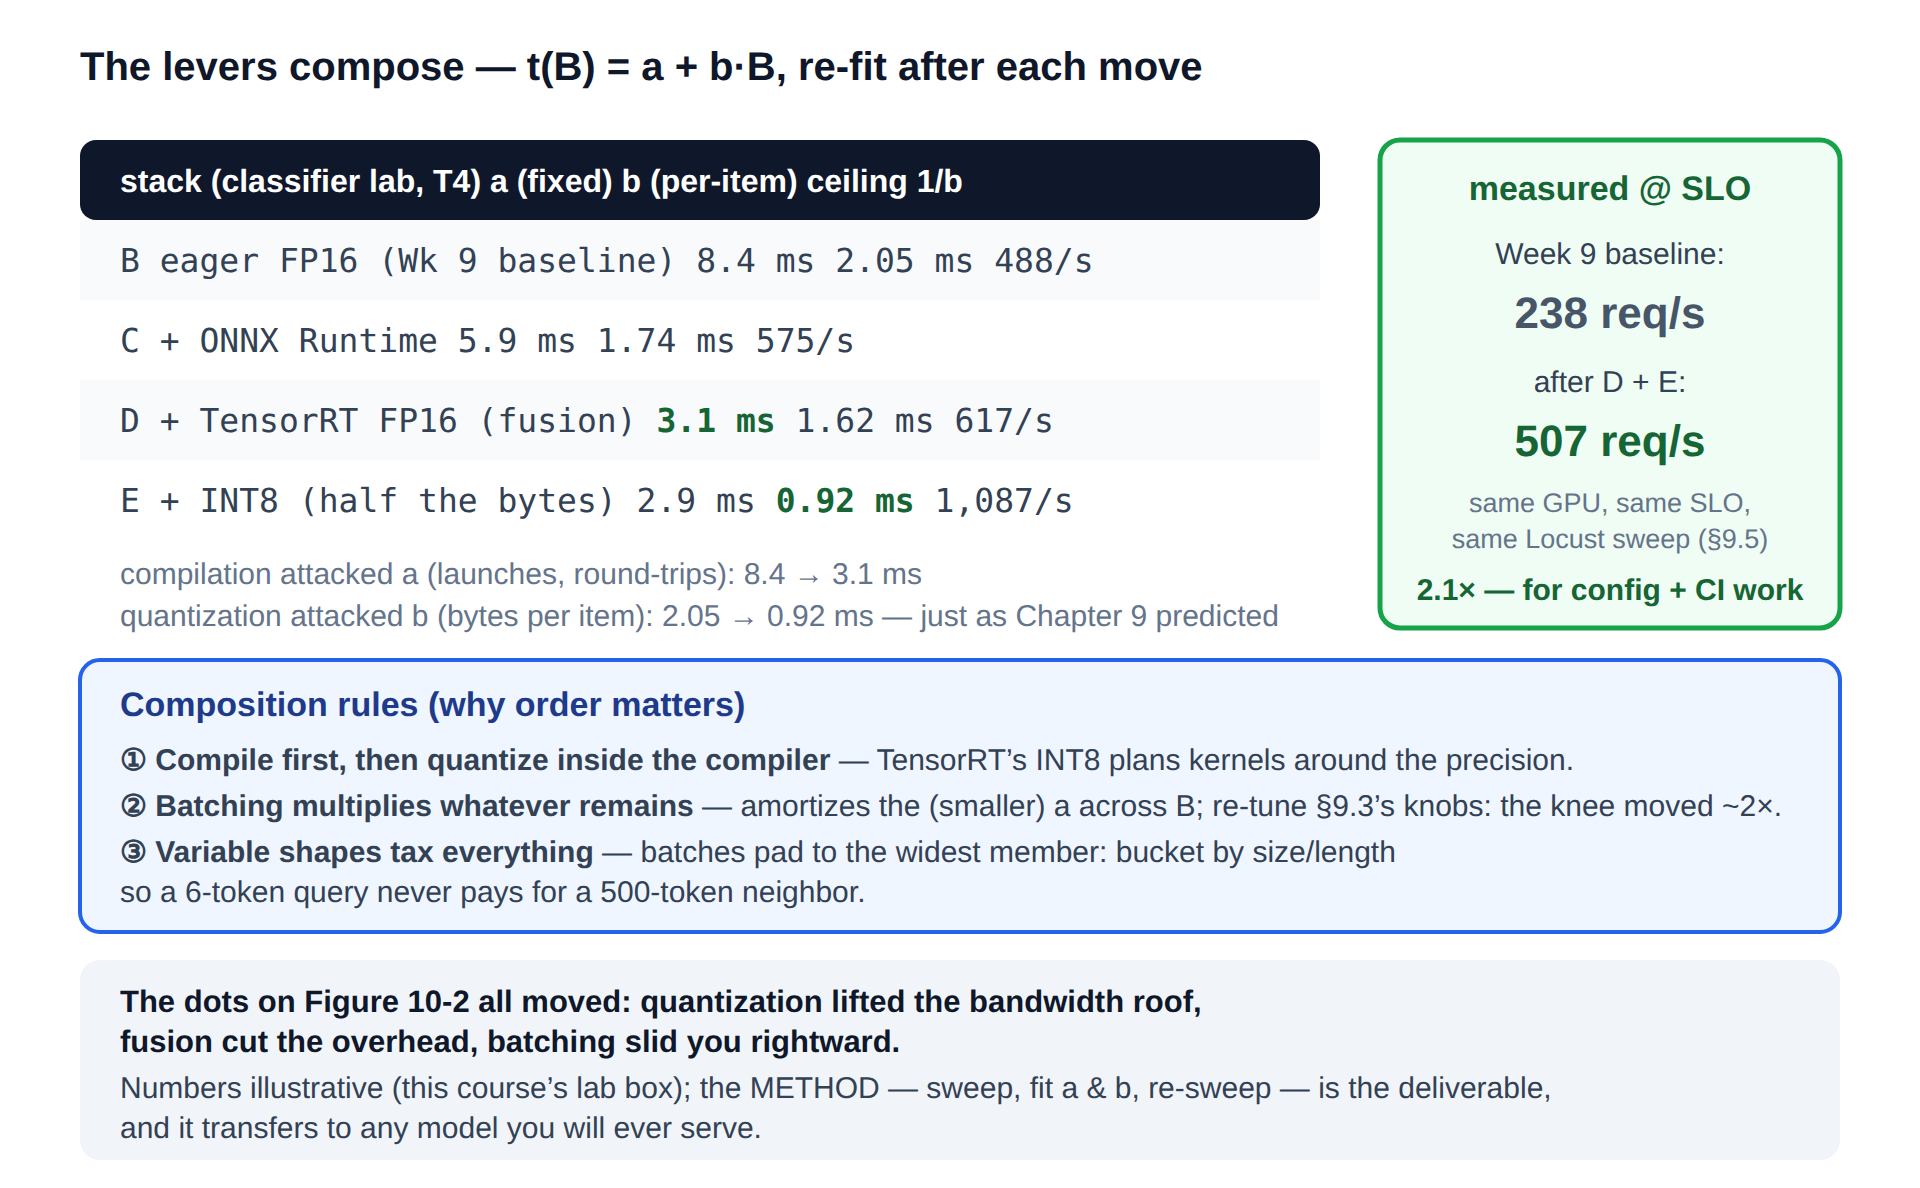
\includegraphics{figures/fig10-6_levers.png}}\\[3pt]
  \figcaption{그림 10-6  여러 수단은 합성된다. 전체 a/b 표, SLO에서 측정한 수치(238 → 507 req/s), 조합 규칙을 보여 준다. 순서가 중요하며 가변 형상은 모든 단계에 비용을 더한다.}
\end{tbbfigure}

\subsection*{배치 처리가 효과를 내는 이유 — 대수로 한 번에 정리한 원리}

강의계획서에서는 이번 주의 셋째 주제를 "동적 배치의 원리"라고 부른다. 두 장에 걸쳐 이를 사용했으니 이제 한 줄로 정리할 수 있다. t(B) = a + b·B를 B로 나누면 \textbf{항목당 비용 c(B) = b + a/B}가 된다. b를 향해 내려가는 쌍곡선이다. 원리는 이것이 전부다. \textbf{배치는 오직 a를 상각하는 기법}이다. 실행, 스케줄링, 가중치 스트림이라는 고정 비용을 B명의 동승자에게 나누지만 b는 건드릴 수 없다. 수익이 줄어드는 까닭도 속설이 아니라 \textit{산술}에 있다. B에서 2B로 늘리면 항목마다 a/2B를 회수하므로 배치를 두 배로 키울 때마다 얻는 이점은 직전의 절반이다. 표 10-3은 최적화된 분류기(a = 2.9, b = 0.92)의 수치를 계산한다.

\begin{tbbtablewrap}
  \begin{tabular}{@{}>{\raggedright\arraybackslash}m{\dimexpr 0.1383\tbltextwidth-2\tabcolsep\relax} >{\raggedright\arraybackslash}m{\dimexpr 0.2128\tbltextwidth-2\tabcolsep\relax} >{\raggedright\arraybackslash}m{\dimexpr 0.2553\tbltextwidth-2\tabcolsep\relax} >{\raggedright\arraybackslash}m{\dimexpr 0.2021\tbltextwidth-2\tabcolsep\relax} >{\raggedright\arraybackslash}m{\dimexpr 0.1915\tbltextwidth-2\tabcolsep\relax}@{}}
  \arrayrulecolor{tbbnavy}\specialrule{1pt}{0pt}{0pt}
  \rowcolor{tbbtablehead}{\centering \bfseries\color{tbbnavy}배치 B} & {\centering \bfseries\color{tbbnavy}t(B) = a + b·B} & {\centering \bfseries\color{tbbnavy}항목당 c(B) = b + a/B} & {\centering \bfseries\color{tbbnavy}이상적 req/s = B/t(B)} & {\centering \bfseries\color{tbbnavy}상한(1/b) 대비} \\
  \arrayrulecolor{tbbnavy}\specialrule{0.7pt}{0pt}{2pt}
  {1} & {3.8 ms} & {3.82 ms} & {262/s} & {24\%} \\
  \arrayrulecolor{tbbtableborder}\hline
  {4} & {6.6 ms} & {1.65 ms} & {608/s} & {56\%} \\
  \arrayrulecolor{tbbtableborder}\hline
  {16} & {17.6 ms} & {1.10 ms} & {908/s} & {84\%} \\
  \arrayrulecolor{tbbtableborder}\hline
  {32} & {32.3 ms} & {1.01 ms} & {990/s} & {91\%} \\
  \arrayrulecolor{tbbtableborder}\hline
  {\textbf{∞}} & {—} & {\textbf{→ b = 0.92 ms}} & {\textbf{→ 1,087/s}} & {100\%} \\
  \arrayrulecolor{tbbnavy}\specialrule{1pt}{2pt}{0pt}
  \end{tabular}\par
  \figcaption{표 10-3  상각 계산(INT8 변형: a = 2.9 ms, b = 0.92 ms). 셋째 열에서 굴곡점이 보인다. "이상적 req/s"는 대기열 처리를 무시하므로 SLO에서 측정한 실제 수치는 이보다 낮다(제7장의 여유 용량).}
\end{tbbtablewrap}

표를 두 가지로 읽으면 앞의 대수가 제값을 한다. 첫째, \textbf{어려운 부분은 "동적"이라는 말이며, 이는 GPU가 아니라 대기열에 관한 용어다.} 트래픽은 한 번에 하나의 요청으로 도착한다. 따라서 §9.3의 배처는 \textit{기다림으로} 상각을 산다. 함께 탈 요청을 기대하며 첫 요청을 max\_queue\_delay만큼 붙잡되, 기다림 + t(B)가 SLO 예산 안에 들어야 한다. 제9장에서 관찰한 자기 조절에는 이제 작동 원리가 생겼다. 부하가 낮으면 거의 비어 있는 상태에서 창이 만료되어 작은 배치가 된다. 유휴 시스템에는 효율이 필요 없으므로 괜찮다. 부하가 높으면 즉시 차서 큰 배치가 되고, 효율이 필요한 바로 그때 나타난다. 둘째, \textbf{최적화는 이제 직관적으로 예상할 수 있는 방향으로 굴곡점을 옮겼다.} a가 8.4에서 2.9 ms로 줄면 \textit{상각할 고정 비용 자체가 적다.} 배치 4에서 이미 상한의 56\%를 얻으며, 최적화 전에는 \textasciitilde{}49\%였다. 배치를 더 깊게 해도 얻는 몫은 얇아진다. 따라서 지연 창을 \textit{줄여} 지연 시간 개선을 취하는 것이 흔히 옳다. 아래 규칙 ②는 주장한 것이 아니라 도출한 결론이다. "최적화 뒤에 조절점을 다시 튜닝하라"는 말이 선택적인 위생 관리가 아닌 이유도 여기에 있다. 같은 두 상수가 움직였기 때문이다.

\subsection*{조합 규칙}

수단을 쌓는 방식은 세 가지 규칙이 지배한다. 이를 모르면 동료 중 누군가는 반드시 같은 실수를 한다. \textbf{규칙 ① — 먼저 컴파일하고 컴파일러 안에서 양자화한다.} TensorRT의 INT8 모드는 정밀도를 \textit{중심으로} 커널을 계획한다. 어느 계층과 융합 그룹을 쓸지, 역양자화(dequantization) 경계를 어디에 둘지 결정한다. 컴파일러가 보지 못한 그래프를 양자화하면 두 도구 모두 눈을 가린 채 일한다. 그래서 사례 10-A의 E행은 두 부품을 따로 붙인 것이 아니라 한 번에 빌드한 "TensorRT INT8"이다. \textbf{규칙 ② — 배치 처리는 남은 것을 곱한다.} 배처는 줄어든 a를 B개 항목에 상각하므로 최적화 후 §9.3의 조절점을 다시 튜닝해야 한다. a = 8.4가 아니라 2.9 ms이면 더 작은 배치가 더 일찍 효율에 도달하고 굴곡점은 \textasciitilde{}2× 더 멀어진다. 처리량이 오르는 동안에도 max\_queue\_delay를 \textit{줄일} 수 있는 경우가 많다. 가정하지 말고 다시 스윕하라. \textbf{규칙 ③ — 가변 형상은 모든 것에 비용을 부과한다.} 배치는 모든 항목을 가장 넓은 형상에 맞춰 패딩한다. 6토큰 쿼리를 500토큰 문서와 같은 배치로 묶으면 500토큰 분량의 작업 비용을 낸다. 해결책은 \textbf{버킷팅(bucketing)}이다. 이미지 해상도나 시퀀스 길이 구간 같은 크기 등급으로 요청을 묶어 패딩(padding) 낭비를 제한한다. 버킷은 컴파일러의 형상 프로파일(§10.4)과 \textit{함께} 설계해야 한다. 버킷과 프로파일은 서로 다른 두 도구에서 본 같은 결정이다. 11주 차에는 이를 논리적 끝까지 밀고 간다. LLM 생성에서는 매 단계마다 모든 시퀀스의 길이가 달라지므로 연속 배치가 필요하다.

보고서에는 정직한 각주가 하나 필요하다. 이 개선은 \textbf{레플리카별 경제성이지 마법이 아니다.} 507 req/s 변형도 여전히 하키 스틱을 따른다. 굴곡점이 옮겨졌을 뿐이다. SLO를 지키려면 여유 용량이 필요하고, 보정을 소홀히 하면 게이트에 실패한다. 여러 수단을 합성한 개선이 플릿의 가격표를 다시 쓴다. 프로젝트 모델이 SLO에서 28 → 57 req/s로 개선되면 제7장이 예고한 그대로 레플리카가 8개 → 4개, 비용이 \$4,762 → \$2,381로 바뀐다. 12주 차 오토스케일링은 이 비용을 다시 절반으로 줄일 차례를 기다리고 있다.

\begin{calloutbox}{tbbpurple}{tbbxF5F3FF}
{\normalsize\bfseries\color{tbbx5B21B6}상자 10-2  나머지 선택지 — 이번 주에 의도적으로 사용하지 않은 수단}\par\vspace{3pt}
이 장의 세 수단에는 공통점이 있다. \textbf{학습 루프가 필요 없다.} 이미 가진 산출물을 대상으로 CI에서 몇 분 안에 실행한다. 더 넓은 선택지는 이 장점을 포기하는 대신 더 크거나 다른 개선을 얻는다. 어떤 방법이 있고 대가가 무엇인지 알아 두자.

\begin{tbbitemize}
  \item \textbf{증류(distillation)}(Hinton et al., 2015): 작은 \textit{학생} 모델이 큰 \textit{교사} 모델의 출력을 모방하도록 학습한다. DistilBERT는 BERT보다 매개변수를 40\% 줄이면서도 성능의 \textasciitilde{}97\%를 유지한 것으로 유명하다. 구조적이고 영구적인 개선이지만, 전체 학습 파이프라인과 데이터 및 수 주의 시간이 필요하다. CI 단계가 아니라 \textit{모델링} 프로젝트다.
  \item \textbf{가지치기(pruning)와 구조적 희소성(structural sparsity)}: 가중치를 완전히 삭제한다. 비구조적 가지치기는 GPU에서 효과를 내는 경우가 드물다. 불규칙한 0은 작업을 건너뛰게 하지 못하기 때문이다. \textbf{2:4 구조적 희소성}은 가중치 네 개마다 두 개를 0으로 만들며 Ampere+ 텐서 코어에서 실제 연산 속도를 두 배로 높인다. 다만 희소화와 미세 조정 주기를 거쳐야 하므로 역시 학습이다.
  \item \textbf{추측 디코딩(speculative decoding)}(11주 차): 작은 모델이 토큰 초안을 만들고 큰 모델이 한 번의 배치 패스로 검증한다. LLM의 토큰별 가중치 스트림을 직접 공격한다. 재학습은 필요 없지만 생성에 특화된 메커니즘이므로 생성 자체가 온전한 주제가 되는 장에서 다룬다.
  \item \textbf{캐스케이드와 조기 종료}: 쉬운 입력은 작은 모델로, 어려운 입력은 큰 모델로 보낸다. \textit{시스템} 차원의 수단이며 제12장의 라우터 영역에 속한다. 게이트도 정확도 델타가 아니라 라우팅 지표다.
\end{tbbitemize}

선택지 어디에서나 규율은 같다. 먼저 진단하고(§10.2), 정직하게 게이트를 적용하며(§10.3), 개선의 원인을 밝힌다(§10.5). 통화만 다를 뿐이다.
\end{calloutbox}

\vspace{3.0pt}

\begin{calloutbox}{tbbpurple}{tbbpurplefill}
{\normalsize\bfseries\color{tbbpurple}생각해 보기}\par\vspace{3pt}
\begin{tbbitemize}
  \item 팀원이 "배치 32에서 INT8이 1.26×밖에 개선하지 못했다. 홍보 자료에는 2×라고 했는데 실망스럽다"고 보고한다. 터미널 기록 10-6의 수치로 배치 32의 속도 향상이 SLO에서의 개선을 과소평가하는 이유를 보여라. t(32)의 비율과 상한의 비율을 계산하면 된다. 대신 보고해야 할 단일 수치는 무엇인가?
  \item 최적화 후 기존 max\_queue\_delay=10 ms 창이 SLO 굴곡점을 지나 포화되는 배치를 모은다. a = 2.9, b = 0.92, SLO 500 ms에서 §9.3의 두 조절점을 다시 튜닝하는 과정을 설명하라. 무엇이 변하고 무엇은 변하지 않는가? 제5장의 memory.max도 다시 측정해야 하는 이유는 무엇인가?
  \item 텍스트 서비스의 길이가 5–800 tokens 범위에서 균일하게 분포한다. 버킷의 수와 경계를 설계하고 이에 맞는 TensorRT 프로파일을 구성하라. 버킷이 있을 때와 없을 때 최악의 패딩 낭비도 계산하라.
\end{tbbitemize}
\end{calloutbox}

\section{실습: 전후 벤치마크 보고서}

이번 실습은 이 장의 내용을 자신의 모델에서 직접 실행한다. 결과물은 프로젝트 평가 기준이 1주 차부터 요구해 온 \textbf{전후 벤치마크 보고서}, 즉 "최적화 전후 비교"다. 그림 10-7의 구조를 보자. 9주 차 스윕은 이미 \textit{이전} 결과다. 이번 주에는 게이트를 적용한 변형을 빌드하고 같은 스윕을 그대로 다시 실행한 뒤, 표를 보고서로 바꾸는 두 문단을 작성한다.

\begin{tbbfigure}
  \adjustbox{max width=0.94\linewidth,max totalheight=0.46\textheight}{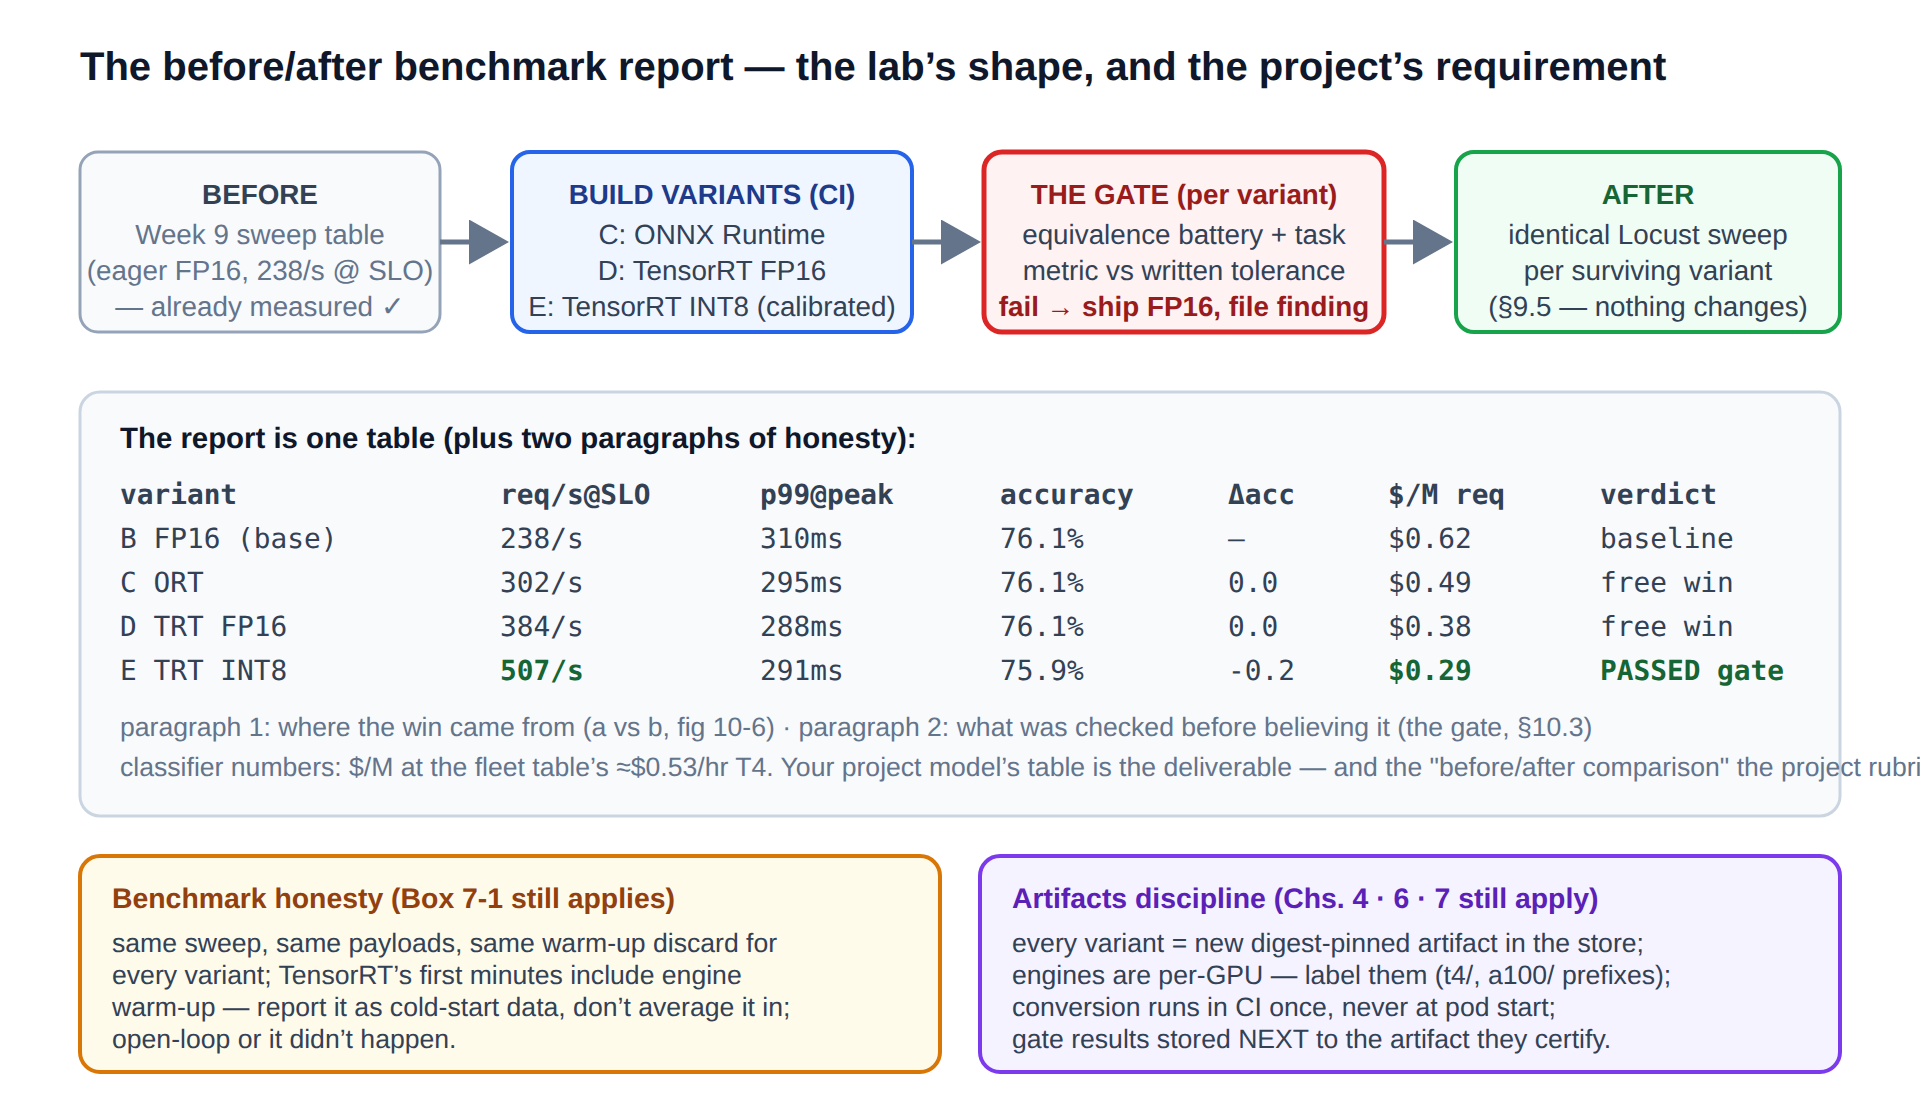
\includegraphics{figures/fig10-7_lab.png}}\\[3pt]
  \figcaption{그림 10-7  실습 파이프라인과 보고서 구조. CI에서 빌드한 각 변형은 게이트와 동일한 스윕을 모두 거친다. 결과물은 표 하나와 정직한 두 문단이다.}
\end{tbbfigure}

\subsection*{일곱 단계}

\begin{tbbitemize}
  \item \textbf{① 진단한다(§10.2).} 자신의 GPU에서 자신의 모델을 대상으로 터미널 기록 10-1의 두 줄을 계산한다. 메모리 벽의 어느 쪽인가? 어떤 수단이 가장 큰 효과를 낼지 어떤 빌드도 하기 \textit{전에} 예측해 적는다. 예측이 틀렸다는 사실을 명확히 드러내도 점수를 얻을 수 있다. 보고서를 통해 무언가 배웠다는 뜻이기 때문이다.
  \item \textbf{② 변형 C를 빌드한다(§10.4).} 내보내기 → CUDA EP를 사용하는 ONNX Runtime 순서로 진행한다. §7.6의 동등성 검사를 실행한다. 이 변형은 거의 정확히 통과해야 한다.
  \item \textbf{③ 변형 D와 E를 빌드한다(§10.4 + §10.3).} 명시적인 형상 프로파일로 TensorRT FP16을 빌드한 뒤, 엄선한 보정 세트로 INT8을 빌드한다. 최근 트래픽에서 500–1,000개의 입력을 뽑되 클래스 \textit{및 게이트가 검사하는 슬라이스}에 걸쳐 층화한다. 세트의 매니페스트와 다이제스트를 calib 캐시 옆에 저장한다. 게이트의 신뢰성은 보정 세트의 문서화 수준과 정확히 같다.
  \item \textbf{④ 각 변형에 게이트를 적용한다(§10.3).} 작업 지표를 미리 명시한 허용 오차와 비교하고 슬라이스를 검사한다. 각 게이트 보고서를 산출물 옆에 저장한다. 게이트에 실패하면 FP16을 배포하고 발견 사항을 기록한다. 이 역시 \textit{완전하며 통과한} 실습 결과다.
  \item \textbf{⑤ 살아남은 각 변형을 스윕한다(§9.5, 변경 없음).} 같은 locustfile, 같은 속도, 같은 워밍업 폐기 구간을 사용한다. TensorRT 엔진 워밍업은 정상 상태 평균에 섞지 않고 콜드 스타트 데이터로 보고한다.
  \item \textbf{⑥ a와 b를 다시 적합한다(§10.5).} 변형마다 시간을 측정한 지점 두 개를 추가하고 모든 개선을 해당 메커니즘에 귀속한다. 귀속 결과가 예상과 다르면 그대로 적는다. 그 문장이 보고서에서 가장 가치 있을 수 있다.
  \item \textbf{⑦ 가격을 다시 계산한다(제7장의 청구서).} SLO에서 측정한 레플리카별 새 수치 → 새 플릿 크기 → 새 월 비용을 제안서에 반영한다. 프로젝트의 비용 이야기는 이제 추정 → 측정(9주 차) → 최적화(10주 차)로 이어지고, 12주 차 오토스케일링을 다음 수단으로 명시해야 한다.
\end{tbbitemize}

"정직한 두 문단"은 실제로 어떤 모습일까? 이미 본 수치를 모두 활용해 분류기용 예시를 작성했다. 문장이 아니라 \textit{구조}를 참고하라.

\begin{calloutbox}{tbbteal}{tbbxF0FDFA}
{\normalsize\bfseries\color{tbbx115E59}사례 10-B  완성된 보고서의 두 문단}\par\vspace{3pt}
\textbf{¶1 — 개선은 어디에서 왔는가.} "최적화로 분류기의 성능은 p99 ≤ 500 ms SLO에서 238 req/s에서 507 req/s로 이동했다(2.1×). T4의 요청 백만 건당 비용으로는 \$0.62 → \$0.29다. 다시 적합한 결과는 개선의 출처를 보여 준다. 컴파일은 디스패치와 실행 오버헤드를 줄여 a를 8.4에서 3.1 ms로 낮췄다. 즉시 실행 연산 \textasciitilde{}175개를 커널 \textasciitilde{}60개로 융합한 §10.4의 계산과 일치한다. 활성값 왕복을 융합해 b도 2.05에서 1.62 ms로 줄였다. 이어 INT8은 텐서 코어 속도가 두 배가 된 덕분에 b를 0.92 ms로 줄였다. ①단계의 예측은 절반만 맞았다. INT8이 바이트를 절반으로 줄이는 효과가 지배할 것으로 예상했지만, 적합 결과 이 모델은 배치 1에서 \textit{실행 병목}이고 배치 16에서는 연산 병목에 가까웠다. INT8의 개선은 바이트가 아니라 연산 속도에서 나왔다. 메커니즘에 대한 예상은 틀렸지만 크기는 맞았다. 다음 모델은 60× 더 크므로 이 차이가 중요하다."

\textbf{¶2 — 믿기 전에 무엇을 확인했는가.} "모든 변형이 §7.6의 동등성 검사를 통과했다. INT8은 벤치마크 \textit{전에} 제안서에 기록한 0.5 pt 허용 오차에 대해 −0.22 pt로 게이트를 통과했다. 보고서는 t4/clf\_int8/gate.json에 저장했다. 슬라이스 검사에서는 \textit{streetcar}가 −1.8 pt로 표시되었다. 보정 매니페스트를 보니 streetcar 이미지가 3장뿐이어서 40장으로 다시 보정했고, 전체 델타는 그대로인 채 해당 슬라이스가 −0.6 pt로 회복되었다. 모든 변형은 동일한 locustfile(다이제스트 9f3c…), 동일한 속도를 사용했고 첫 60 s를 폐기했다. TensorRT 엔진 로드는 정상 상태 평균에 넣지 않고 콜드 스타트로 보고했다. 엔진에는 t4/ 접두사가 있으며 팀의 A10G 한 대는 설계대로 이를 거부한다."

\textit{이 글이 좋은 평가를 받는 이유는 ¶1의 모든 수치를 메커니즘에 귀속하고 ¶2의 모든 주장을 저장된 산출물로 확인할 수 있기 때문이다. 틀린 예측 하나도 숨기지 않고 명시했다. 채점자와 미래의 팀원, 14주 차 사고 검토자가 바로 이런 내용을 읽는다.}
\end{calloutbox}

\vspace{3.0pt}

\begin{calloutbox}{tbbred}{tbbxFEF2F2}
{\normalsize\bfseries\color{tbbx991B1B}상자 10-1  보고서의 위험 신호(공개된 채점자 점검표)}\par\vspace{3pt}
\begin{tbbitemize}
  \item \textbf{게이트 결과가 나란히 없는 속도 향상} — 빠르지만 틀린 모델은 최적화가 아니다.
  \item \textbf{변형마다 서로 다른 스윕}(속도, 페이로드, 워밍업) — 비교 자체가 결과물이므로 지켜야 한다.
  \item \textbf{배치 N 지연 시간 비율을 "속도 향상"으로 제시} — 중요한 수치는 SLO에서의 req/s(유효 처리량)와 a/b 귀속이다.
  \item 경로나 메타데이터에 \textbf{GPU 좌표가 없는 엔진 산출물} — 언젠가는 반드시 잘못된 플릿에 배포된다. 제4장의 다이제스트 교훈을 하드웨어에 적용한 사례다.
  \item \textbf{"시작할 때 파드 안에서 양자화했다"} — 변환은 CI에서 한 번 수행하고 게이트를 적용한다(§7.6, §10.4). 콜드 스타트 경로는 계속 신성하게 지킨다.
\end{tbbitemize}
\end{calloutbox}

\vspace{3.0pt}

제출물은 표 하나와 두 문단(개선이 어디에서 왔는가, 믿기 전에 무엇을 확인했는가)으로 구성한 보고서, 변형별 게이트 출력, 다시 적합한 상수, 갱신한 제안서 비용 항목이다. 결제 내역 스크린샷도 계속 제출한다. 엔진 빌드를 포함한 일반적인 실습 비용은 T4 시간 기준 \textasciitilde{}\$3–4다.

\begin{calloutbox}{tbbpurple}{tbbpurplefill}
{\normalsize\bfseries\color{tbbpurple}생각해 보기}\par\vspace{3pt}
\begin{tbbitemize}
  \item 보고서의 첫 문단을 "§10.2의 내용에 따라 컴파일이 지배할 것으로 예상한다..."와 같은 가설 형태로 미리 작성한 뒤 ⑥단계가 끝나면 채점하라. 자신의 모델은 실제로 메모리 벽의 어느 쪽에 있었는가?
  \item INT8 변형이 0.5 pt 허용 오차에 대해 0.9 pt로 게이트에 실패한다. 네 가지 선택지를 비용이 늘어나는 순서대로 나열하라. 더 나은 보정 → 채널별/그룹별 세분성 → 가중치 전용/혼합 정밀도 → QAT 순이다. 각 단계에서 다음 단계로 넘어갈 근거도 제시하라.
  \item 최적화 모델은 제2장의 플릿 답을 바꾼다. T4 한 대당 507 req/s일 때 가격이 ≈5×이고 이 모델 처리량이 ≈2.5×인 A100이 이 분류기 서빙에서 유리한 부하가 하나라도 있는가? 계산으로 보여라. A100이 유리해지는 워크로드도 제시하라. 힌트는 §10.2의 메모리 벽이다.
\end{tbbitemize}
\end{calloutbox}

\namedsection{요약}{열다섯 가지 핵심 내용}

\qitem{1}{\textbf{최적화란 같은 SLO에서 요청당 비용을 낮추는 것이다.} 사례 10-A에서는 하나의 모델과 하나의 GPU를 네 스택에서 실행했다. 같은 p99에서 28 → 57 req/s, 백만 건당 \$7.94 → \$3.90이 되었고, 제7장이 예고한 대로 플릿은 레플리카 8개 → 4개, \$4,762 → \$2,381/month로 줄었다. 모델의 지식은 전혀 바뀌지 않았다.}

\qitem{2}{\textbf{우리는 평생 손실 압축(lossy compression)을 믿어 왔다.} 8-bit μ-law 전화(1962), JPEG (1992), MP3 (1993)는 신호 소비자에게 필요한 것을 찾아 나머지에 비용을 내지 않는 방식이다. 양자화는 모델 자체의 결정을 소비자로 삼아 이 패턴을 적용한다. 학습에는 작은 경사 단계를 위한 세밀한 눈금이 필요하지만 추론에서는 반올림 뒤에도 최댓값의 위치나 토큰만 살아남으면 된다. 평평한 최솟값이 이를 가능하게 한다.}

\qitem{3}{\textbf{메모리 벽은 가장 중요한 진단 기준이다.} T4는 65 TFLOPS를 수행하지만 320 GB/s만 이동하므로 바이트당 \textasciitilde{}200 FLOP이 필요하다. 이 능선과 비교한 산술 집약도(FLOPs/byte)가 모든 것을 결정한다. 서빙 배치에서 대부분의 추론은 메모리 병목이므로 비용은 연산이 아니라 바이트다. 터미널 기록 10-1처럼 프로파일러 없이 두 줄로 진단할 수 있다.}

\qitem{4}{\textbf{루프라인에서 각 수단은 기하학적 의미를 지닌다.} 배치는 가중치를 B개 항목에 재사용해 오른쪽으로 이동시키고, 양자화는 가중치당 바이트를 줄여 대역폭 지붕을 높이며, 컴파일은 융합 커널로 활성값이 VRAM에 가지 않게 해 벽의 비용을 중복해서 내지 않는다. 능선은 카드마다 다르다(표 10-1). L4는 약 400이고 A100 프리미엄의 대부분은 대역폭이다. 세대마다 벽이 높아지므로 바이트는 가치가 오르는 통화다.}

\qitem{5}{\textbf{바이트는 세 가지 속도의 여정을 거친다(제6장의 약속을 지켰다).} 객체 스토어 → 호스트 페이지 캐시(파드마다 한 번) → PCIe의 고정 H2D(\textasciitilde{}12 GB/s, 프로세스마다 한 번) → VRAM에서 연산 장치(300 GB/s, 모든 패스)로 이동한다. PCIe는 VRAM보다 \textasciitilde{}25× 느리고 페이지 가능 복사는 이를 다시 절반으로 줄인다. 따라서 가중치는 시작 시 한 번만 건너고 요청별 텐서는 고정 버퍼와 비동기 복사를 사용한다. nvidia-smi dmon의 PCIe 열은 진단의 셋째 줄이다.}

\qitem{6}{\textbf{부동소수점은 관대하고 정수는 위임한다.} 부동소수점은 지수로 값마다 자체 스케일을 조정하지만 정수는 텐서 전체가 보정된 스케일 하나를 공유한다. 이것이 §10.3의 모든 함정의 근원이다. FP16은 범위를 희생해 학습 시 손실 스케일링이 필요하고, BF16은 FP32의 범위를 유지해 학습에서 각광받았다. FP8 (Hopper/Ada)은 정수 수준의 저장 비용에 자체 스케일링을 남겼다. INT8×INT8의 합은 INT32에 누적되므로 정확도 저하는 언제나 눈금 배치 문제이지 오버플로 문제가 아니다.}

\qitem{7}{\textbf{양자화는 거친 자를 잘 배치하는 일이다.} q = round(w/scale) + zero\_point에서 비대칭 zero\_point는 자를 옮겨 ReLU 이후 범위에서 눈금을 낭비하지 않게 한다. 가중치에는 채널별 스케일을 쓴다. 하나의 공유 스케일은 ±0.05 채널에 21\% 오차를 내지만 자체 자는 0.4\%만 낸다. INT4 LLM은 그룹별 스케일을 쓴다. 보정은 최솟값–최댓값, 백분위수 또는 KL로 활성값 범위를 정하며, 보정의 품질이 곧 양자화 품질이다. PTQ는 CI에서 몇 분이면 되고 PTQ가 게이트에 실패하면 QAT로 확대한다.}

\qitem{8}{\textbf{두 가지 함정이 있다.} 채널마다 범위가 다르므로 채널별 스케일이 필요하고, 트랜스포머 활성값에는 이상치가 숨어 있다(LLM.int8(), 2022). 그래서 LLM은 기본적으로 가중치 전용 양자화를 쓰며, 평활화나 혼합 정밀도를 적용하기도 한다. CNN급 실습 모델은 전체 W8A8을 견딘다.}

\qitem{9}{\textbf{게이트는 손실 변환에 정당성을 부여한다.} 작업 지표를 벤치마크 전에 명시한 허용 오차와 비교하고 슬라이스를 검사한다. 출력은 게이트 보고서를 나란히 둔 새 다이제스트 고정 산출물이다. 게이트에 실패해 FP16을 배포하는 것은 통과한 결과지만, 게이트 없이 배포하면 "모델이 이상해졌다"는 티켓이 생긴다.}

\qitem{10}{\textbf{컴파일러는 a를 줄인다. 융합, 폴딩, 레이아웃 계획, 오토튜닝이 핵심이다.} 네 번 대신 한 번만 실행하고 활성값 왕복을 없애며, 빌드 시점에 실제 GPU와 형상에서 커널을 벤치마크한다. 대가는 좁은 범위다. 엔진은 GPU별, 형상 프로파일별 산출물이며 t4/ 접두사가 꼭 필요하다. torch.compile의 워밍업은 콜드 스타트 경로에 붙는다.}

\qitem{11}{\textbf{세 컴파일러는 하나의 패턴을 따른다.} ONNX Runtime은 플러그형 EP를 갖춘 이식성 있는 중간 지점이고, TensorRT는 가장 빠르지만 가장 좁으며 빌더 안에서 INT8을 보정한다. torch.compile은 즉시 실행에 자연스러운 런타임 JIT다. 가중치 병목 디코드, 제각각인 형상, 사용자 정의 연산에서는 컴파일이 예상대로 기대에 못 미치므로 먼저 진단해야 한다.}

\qitem{12}{\textbf{배치는 오직 a를 상각한다.} c(B) = t(B)/B = b + a/B는 b를 향해 내려가는 쌍곡선이다. B를 두 배로 늘릴 때마다 얻는 이점은 직전의 절반이므로 굴곡점은 속설이 아니라 산술에서 나온다. 표 10-3에서 배치 4는 최적화 상한의 56\%를 이미 얻는다. \textit{동적}이라는 말은 대기열 측면을 뜻한다. SLO 예산 안에서 동승자를 기다리는 제한된 시간을 효율과 맞바꾸고, 부하에 따라 스스로 조절한다.}

\qitem{13}{\textbf{조합 규칙을 지켜야 한다.} 먼저 컴파일하고 컴파일러 안에서 양자화한다. 배치 처리는 남은 것을 곱하므로 §9.3의 조절점을 다시 튜닝한다. 굴곡점이 움직였고 상각할 a가 줄어 지연 창을 흔히 \textit{줄일} 수 있다. 가변 형상은 모든 것에 비용을 부과하므로 형상 프로파일과 함께 크기별 버킷을 설계한다.}

\qitem{14}{\textbf{다시 적합한 결과가 보고서다.} t(B) = a + b·B에서 변형마다 두 번 실행한다. 컴파일의 흔적은 a (8.4 → 3.1 ms), 양자화의 흔적은 b (2.05 → 0.92 ms)에 나타난다. 상한은 488 → 1,087/s, 측정값은 SLO에서 238 → 507 req/s가 된다. 원인 귀속이 막대그래프를 엔지니어링으로 바꾼다.}

\qitem{15}{\textbf{최적화는 하드웨어의 가격표를 다시 쓴다.} 대표 70B 모델은 INT4에서 140 → \textasciitilde{}35 GB로 줄고, A100이 필요하던 모델이 T4 플릿에 들어간다. 제2장의 표와 제5장의 nodeSelector에는 새로운 정답이 생긴다. 정밀도를 바꿀 때마다 플릿 표를 다시 읽어야 한다.}

\namedsection{연습문제}{}

\subsection*{A. 객관식}

\qitem{1}{FP16의 7B 모델(14 GB의 가중치)이 대역폭 700 GB/s인 GPU에서 배치 1로 토큰을 생성한다. 토큰당 지연 시간 하한과 그 원인을 가장 잘 추정한 것은 무엇인가?}

\begin{tbboptions}
  \item ① \textasciitilde{}2 ms — 커널 실행 오버헤드        ② \textasciitilde{}20 ms — 토큰마다 가중치를 한 번 스트리밍해야 한다(14 GB ÷ 700 GB/s)
  \item ③ \textasciitilde{}0.1 ms — 연산이 단순하다        ④ 프로파일러 없이는 추정할 수 없다
\end{tbboptions}

\qitem{2}{가중치를 FP16에서 INT8로 양자화할 때 직접 생기지 않는 변화는 무엇인가?}

\begin{tbboptions}
  \item ① 패스마다 스트리밍하는 바이트가 절반이 된다        ② 가중치용 VRAM이 절반이 된다
  \item ③ INT8 지원 GPU에서 텐서 코어 연산 속도가 두 배가 된다        ④ 모델 정확도가 높아진다
\end{tbboptions}

\qitem{3}{트랜스포머 활성값 이상치가 단순한 W8A8 양자화를 깨뜨리는 이유는 무엇인가?}

\begin{tbboptions}
  \item ① INT8은 음수를 표현할 수 없다
  \item ② 소수의 큰 값이 스케일을 늘려 일반 값을 거의 0에 가깝게 반올림하게 한다
  \item ③ 활성값은 요청마다 변하므로 어떤 스케일도 존재할 수 없다
  \item ④ GPU는 활성값을 FP64로 처리한다
\end{tbboptions}

\qitem{4}{가장 큰 이점을 얻기 위한 올바른 작업 순서는 무엇인가?}

\begin{tbboptions}
  \item ① ONNX 파일을 양자화한 뒤 TensorRT에 건넨다        ② 컴파일러가 정밀도에 맞춰 커널을 계획하도록 INT8 모드 + 보정으로 TensorRT 엔진을 빌드한다
  \item ③ 개선은 독립적이므로 순서는 중요하지 않다        ④ 먼저 배치하고 컴파일한 뒤 파드 시작 시 양자화한다
\end{tbboptions}

\qitem{5}{다시 적합한 결과 변형 X에서 b는 변하지 않고 a만 8.4 → 3.2 ms로 줄었다. 변형 X일 가능성이 가장 큰 것은 무엇인가?}

\begin{tbboptions}
  \item ① INT8 양자화        ② 그래프 컴파일(융합 + 오토튜닝)
  \item ③ 더 큰 배치 크기        ④ 더 빠른 토크나이저
\end{tbboptions}

\qitem{6}{T4에서 maxShapes batch=32로 빌드한 TensorRT 엔진이 A10G에서 배치 48을 받는다. 어떤 일이 일어나는가?}

\begin{tbboptions}
  \item ① 조금 느리지만 실행된다        ② 배치를 조용히 잘라 낸다
  \item ③ 엔진용 GPU가 잘못되었고 형상도 프로파일 밖이므로 두 조건 모두에서 실패한다. 엔진은 GPU별, 프로파일별 산출물이다
  \item ④ TensorRT가 즉석에서 엔진을 다시 빌드한다
\end{tbboptions}

\qitem{7}{게이트의 허용 오차("≤ 0.5 pt top-1 loss")를 벤치마크 전에 명시해야 하는 이유는 무엇인가?}

\begin{tbboptions}
  \item ① 규정이 요구한다        ② 그렇지 않으면 관찰된 손실을 보고 나서야 "허용 가능"의 뜻을 정하게 된다. 측정 전에 SLO를 약속하는 것에 대응하는 정확도 규율이다(§7.4)
  \item ③ TensorRT가 빌드 플래그로 사용한다        ④ 보고서가 짧아진다
\end{tbboptions}

\qitem{8}{최적화 후(a: 8.4→2.9, b: 2.05→0.92) §9.3의 배치 조절점에 관한 설명으로 옳은 것은 무엇인가?}

\begin{tbboptions}
  \item ① 영향을 받지 않는다. 배치 처리는 직교한다
  \item ② 굴곡점이 바깥으로 \textasciitilde{}2× 이동하고 더 작은 배치가 더 빨리 효율에 도달하므로 두 조절점과 제5장의 memory.max를 모두 다시 스윕해야 한다
  \item ③ max\_queue\_delay를 두 배로 늘려야 한다        ④ max\_batch\_size에는 더 이상 VRAM 상한이 없다
\end{tbboptions}

\subsection*{B. 단답형}

\qitem{1}{320 GB/s GPU에서 배치 1로 실행하는 1.5 GB INT8 모델의 두 줄짜리 진단(바이트 하한과 FLOP 하한)을 제시하고 결론을 내려라.}

\qitem{2}{게이트의 세 부분과 이를 통과한 모든 변형에 적용되는 산출물 규칙을 서술하라.}

\qitem{3}{LLM에서는 가중치 전용 INT4가 기본인 반면 실습의 CNN에서는 전체 W8A8이 동작하는 이유는 무엇인가? 모델 계열마다 한 문장으로 답하라.}

\qitem{4}{TensorRT의 "최적화 프로파일"이 무엇이며 어떤 운영 약속을 표현하는지 설명하라.}

\qitem{5}{PTQ와 QAT를 각각 한 문장으로 설명하고, 첫 방법에서 둘째 방법으로 확대하는 조건을 제시하라.}

\qitem{6}{FP16에서 ReLU의 산술 집약도(arithmetic intensity)를 계산하고, 이 수치로 그래프 컴파일러가 ReLU에 별도 커널을 주지 않는 이유를 설명하라.}

\subsection*{C. 서술형}

\qitem{1}{가상의 서비스에 대해 "네 가지 비용" 분석을 작성하라. A100 (weights 26 GB FP16, 2,000 GB/s, 312 TFLOPS)에서 배치 1로 LLM을 디코드한다. 메모리와 연산 하한을 계산하고, 이 장의 수단 중 무엇이 가장 큰 효과와 가장 작은 효과를 낼지 이유와 함께 예측하라. 11주 차 연속 배치가 이들 수단으로는 얻을 수 없는 무엇을 추가하는지도 설명하라.}

\qitem{2}{제도로서 게이트를 옹호하라. PM은 "정확도 0.2 points를 대가로 \$2,400/month를 아낄 수 있는데 당연히 배포해야지, 왜 이런 절차가 필요한가?"라고 묻는다. 허용 오차가 수치보다 먼저 정해지는 이유, 집계값이 보호할 수 없는 무엇을 슬라이스 검사가 보호하는지, 14주 차 사고에서 다이제스트 고정 산출물 + 저장된 게이트 보고서가 주는 이점, PM이 실제로 옳은 지점을 포함해 답하라.}

\qitem{3}{자신의 프로젝트 모델을 위한 전체 최적화 파이프라인을 CI로 설계하라. 단계(내보내기, 빌드, 보정, 게이트, 스윕, 다시 적합, 승격), 산출물과 저장소 레이아웃(제6장), 커밋마다 실행할 작업과 릴리스마다 실행할 작업, 두 실패 경로(게이트 실패, 스윕 회귀)와 각각의 결과를 포함하라. 둘째 GPU 유형이 플릿에 들어오면 어느 단계가 달라지는지도 적어라.}

\qitem{4}{경제성에 관한 글을 작성하라. 최적화 후 분류기는 T4 한 대(≈\$0.53/hr, 표 2-3)에서 507 req/s를 처리한다. 요청 백만 건당 새 비용을 계산한 뒤 같은 모델에서 처리량이 2.5×라고 가정한 A100의 손익분기 가격을 구하라. 메모리 벽을 이용해 메모리 병목 LLM에서는 A100의 이점이 더 커지는 이유를 설명하고, 플릿 권장안과 제5장 nodeSelector에 미치는 영향으로 결론지어라.}

\namedsection{정답과 해설}{}

\subsection*{A. 객관식}

\qitem{1}{\textbf{②} 생성되는 토큰마다 14 GB의 가중치 전체가 연산 장치를 통과해야 한다. 14 ÷ 700 GB/s = 20 ms다. 더 빠른 연산으로도 넘을 수 없는 하한이며, 배치 1 디코드가 루프라인 맨 왼쪽에 놓이는 이유다. (§10.2)}

\qitem{2}{\textbf{④} 양자화는 손실 변환이다. 게이트는 개선을 기대하기 위해서가 아니라 손실의 범위를 제한하기 위해 존재한다. 드물게 우연한 정규화 효과가 있었다는 일화는 엔지니어링 계획이 아니다. ①–③은 정확히 양자화 메커니즘이다. 바이트와 VRAM이 줄고 정수 연산이 빨라진다. (§10.3)}

\qitem{3}{\textbf{②} 드문 스파이크 하나가 자를 늘린다. 256개 눈금이 ±100에 퍼지면 일반적인 ±1 값에는 눈금 몇 개만 남아 뭉개진 값으로 반올림된다. 그래서 트랜스포머에는 가중치 전용 양자화, 평활화 또는 혼합 정밀도를 쓴다. (§10.3)}

\qitem{4}{\textbf{②} 규칙 ①에 따라 컴파일러가 정밀도를 알아야 융합 INT8 커널과 역양자화 경계를 계획할 수 있다. 컴파일러가 보지 못하게 미리 양자화하거나 시작 시점에 양자화하면(④, 콜드 스타트에도 해롭다) 두 도구를 모두 낭비한다. (§10.5)}

\qitem{5}{\textbf{②} a는 패스마다 드는 고정 비용인 실행, 왕복, 폴딩 기회이며 컴파일러가 주로 다루는 영역이다. 양자화는 주로 항목당 바이트와 연산을 뜻하는 b에 나타난다. 다시 적합하는 이유가 바로 이처럼 원인을 귀속하기 위해서다. (§10.5)}

\qitem{6}{\textbf{③} 엔진은 한 GPU 세대에 오토튜닝한 커널과 약속된 형상 범위를 인코딩한다. 둘 중 하나라도 어기면 실행을 거부하거나 아예 로드되지 않는다. 산출물 경로에 하드웨어 좌표를 넣는 이유다. (§10.4)}

\qitem{7}{\textbf{②} 결과를 본 뒤 정의한 허용 오차는 허용 오차가 아니라 합리화다. 약속이 측정보다 앞서야 한다는 점에서 SLO와 같은 규율이다. (§10.3, §7.4)}

\qitem{8}{\textbf{②} a가 작아지면 배치가 상각할 오버헤드가 줄어 효율에 더 일찍 도달하고 전체 곡선이 압축된다. 굴곡점은 req/s 기준으로 더 바깥에 놓인다. 두 조절점과 memory.max의 근거가 되는 최악의 메모리 측정을 모두 다시 살펴봐야 한다. (§10.5, 제5장)}

\subsection*{B. 단답형}

\qitem{1}{바이트: 1.5 GB ÷ 320 GB/s ≈ 패스당 \textbf{4.7 ms}의 하한이다. FLOP: \textasciitilde{}1.5B params × 2 ≈ 3 GFLOP ÷ 65 TFLOPS ≈ \textbf{0.05 ms}다. 결론은 \textasciitilde{}100× 메모리 병목이므로 연산이 아니라 바이트를 줄이는 데 투자해야 한다. 추가 양자화와 배치 처리가 해당한다. (§10.2)}

\qitem{2}{① 별도 보관 세트에서 기준 모델과 비교한 작업 지표, ② 실행 전에 명시한 허용 오차, ③ 집계값이 손상을 감추는 곳의 슬라이스 검사다. 통과한 출력은 게이트 보고서를 옆에 저장한 \textbf{새 다이제스트 고정 산출물}이어야 하며 제자리에서 변경하지 않는다. (§10.3)}

\qitem{3}{LLM: 활성값에 자를 늘리는 스파이크인 이상치가 있으므로 활성값은 FP16으로 두고, 어차피 바이트를 지배하는 가중치만 INT4로 낮춘다. CNN: 활성값이 온순한 종 모양 분포이므로 전체 W8A8이 게이트를 통과하고 정수 연산 속도도 얻는다. (§10.3)}

\qitem{4}{엔진을 빌드할 때 사용한 min/opt/max 형상 범위이며 무엇을 전송할지에 관한 약속이다. 범위 안에서는 오토튜닝한 커널을 쓰고 밖에서는 거부한다. 운영상 §10.5의 버킷팅과 연결되므로 버킷과 프로파일은 하나의 결정이다. (§10.4)}

\qitem{5}{PTQ는 학습 후 보정 데이터에서 스케일을 고르며 학습 루프 없이 몇 분이면 된다. QAT는 미세 조정 중 반올림을 모사해 네트워크가 적응하게 하므로 학습 비용이 든다. PTQ가 명시된 게이트에 실패하고 정밀도 개선이 학습 파이프라인 보유 비용을 정당화할 때 QAT로 확대한다. (§10.3)}

\qitem{6}{원소당 1 FLOP ÷ (읽기 2 B + 쓰기 2 B) = \textbf{0.25 FLOP/byte}다. T4의 능선보다 \textasciitilde{}800× 낮아 ReLU는 어떤 하드웨어에서도 메모리 속도로 실행된다. 독립 ReLU 커널은 순수한 왕복 비용이므로 컴파일러가 값을 생성하는 연산의 에필로그에 융합해 바이트를 완전히 없앤다. (§10.2, §10.4)}

\subsection*{C. 서술형(채점 기준)}

\qitem{1}{하한: 메모리는 26 ÷ 2,000 GB/s = \textbf{13 ms/token}, 연산은 \textasciitilde{}13 GFLOP ÷ 312 TFLOPS ≈ 0.04 ms이므로 \textasciitilde{}300× 메모리 병목이다. 예측: 가중치 전용 양자화가 가장 큰 효과를 내며 INT4는 하한을 \textasciitilde{}3.3 ms로 줄인다. 융합은 가중치 스트림을 건드릴 수 없어 컴파일의 효과가 가장 작다. 동시 시퀀스가 있을 때만 배치가 도움이 된다. 연속 배치는 길이와 단계가 다른 시퀀스 사이에 그 동시성을 만들어 스트리밍한 가중치를 매 단계 상각한다. §9.3의 가정을 복구하며 vLLM이 존재하는 이유다. (§§10.2–10.5, 11주 차)}

\qitem{2}{좋은 답은 다음 내용을 포함한다. 허용 오차가 수치보다 먼저 정해져야 바람에 이끌린 결정을 피할 수 있다(§7.4의 규율). 슬라이스는 제품을 지탱하는 클래스가 평균에 묻히지 않게 보호한다. 사고 중에는 다이제스트 + 저장된 게이트 보고서가 "모델이 바뀌었고 검사를 거쳤는가?"에 몇 분 안에 답하며 제13장의 롤백에 필요하다. 최종 결정이 제품 차원의 절충이라는 점에서는 PM이 옳다. 게이트는 이를 \textit{근거 있는} 절충으로 만들며, 허용 오차는 배포 전에 공개적으로 다시 협의할 수 있다. (§10.3)}

\qitem{3}{포함할 내용: 커밋마다 내보내기 + 동등성 검사, 릴리스마다 GPU 유형별 엔진 빌드 + 보정 + 게이트를 실행한다. 둘째 플릿 구성원이 들어오면 행렬이 두 배가 된다. 스윕 + 다시 적합은 일정에 따라 또는 릴리스마다 실행한다. 승격은 가중치 옆에 게이트 산출물을 둔 저장소 이동이며 t4/, a100/ 접두사를 쓴다. 게이트 실패 → 이전 정밀도 배포 + 발견 사항 기록, 스윕 회귀 → 승격 차단 후 a/b 귀속으로 변형을 이분 탐색한다. 새 GPU가 들어오면 엔진을 다시 빌드하고, 수치가 달라질 수 있으므로 게이트와 스윕을 다시 실행한다. ONNX를 이식 가능한 단일 진실 공급원으로 유지해야 하는 이유다. (§§10.3–10.6, 제4/6장)}

\qitem{4}{분류기: \$0.53 ÷ (507 × 3,600) × 10⁶ ≈ \textbf{\$0.29/M}이다. 처리량이 2.5× (1,268/s)일 때 A100의 손익분기 가격은 0.53 × 2.5 ≈ \textbf{\$1.33/hr} 아래다. 온디맨드(on-demand) 실제 가격 \$3–5의 3분의 1 수준이므로(표 2-3) 연산 비중이 충분한 이 CNN에는 T4가 유리하다. 메모리 병목 LLM에서는 FLOP이 아니라 A100의 6× 대역폭이 배수가 되고 처리량이 대역폭에 거의 비례하므로 같은 계산이 대형 카드 쪽으로 뒤집힌다. 플릿 권장안은 분류기를 T4 레이블에, LLM을 A100 레이블에 두는 것이며 nodeSelector 분할에 비용 근거가 생긴다. (§10.2, §10.6, 제2/5장)}

\namedsection{더 읽을거리}{}

\textbf{[이번 주]}로 표시한 자료는 실습을 직접 뒷받침하고, \textbf{[N주 차]}는 나중에 도움이 될 자료를 뜻한다.

\begin{tbbitemize}
  \item \textbf{[이번 주] TensorRT Developer Guide — "Working with INT8" and "Optimization Profiles"} — 터미널 기록 10-4의 권위 있는 설명이다. 보정, 계층별 정밀도 결정, 형상 약속 메커니즘을 다룬다. 그림 10-5와 함께 읽어 보자.
  \item \textbf{[이번 주] ONNX Runtime 문서 — Graph Optimizations and Execution Providers} — "공짜" 1.4×가 실제로 수행한 작업을 설명한다. 최적화 수준의 단계와 EP가 TensorRT 등을 포함한 하위 그래프를 위임하는 방식을 다룬다.
  \item \textbf{S. Williams, A. Waterman, D. Patterson, "Roofline: An Insightful Visual Performance Model," CACM 2009} — 원래의 루프라인 논문이다. §10.2는 이를 서빙에 맞게 요약했다. 짧고 시간이 지나도 유효하다. GPU가 지금 겪는 문제에 이름을 붙인 CPU 시대의 네 쪽짜리 논문 \textbf{Wulf \& McKee, "Hitting the Memory Wall" (1995)}도 함께 읽어 보자.
  \item \textbf{J. Dettmers et al., "LLM.int8(): 8-bit Matrix Multiplication for Transformers at Scale" (2022)} — 활성값 이상치의 발견을 보기 드물게 명료하게 설명한다. §10.3에서 LLM의 기본값이 가중치 전용인 이유다. 재스케일링 해결책은 \textbf{Xiao et al., "SmoothQuant" (2022)}에서 이어서 볼 수 있다.
  \item \textbf{[11주 차] Frantar et al., "GPTQ" (2022) · Lin et al., "AWQ" (2023)} — 다음 주 vLLM으로 서빙할 모델의 기반이 되는 4비트 가중치 전용 기법이다. 이 장에서 배운 그룹별 스케일 용어를 알면 읽기 쉽다.
  \item \textbf{PyTorch 문서 — torch.compile(Inductor) 튜토리얼과 문제 해결} — 그래프 단절, 재컴파일 조건, 콜드 스타트 예산이 부담할 워밍업 비용 등 즉시 실행에 자연스러운 경로의 실제 동작을 설명한다.
  \item \textbf{[이번 주, 재미] 어떤 이미지 편집기의 JPEG 품질 슬라이더} — 사진에서 100부터 10까지 내려 보며 직접 차이를 알아채는 지점을 찾아보자. 자신의 시각 피질에 보정 + 게이트를 수행하는 셈이며, 실습은 여기에 허용 오차를 명시한 같은 실험이다.
\end{tbbitemize}

\vspace{5.0pt}

\begin{calloutbox}{tbbblue}{tbbbluefill}
{\normalsize\bfseries\color{tbbblue}다음 장 — 제11장: LLM 서빙}\par\vspace{3pt}
지금까지 최적화한 모든 시스템은 한 덩어리로 답했다. 요청이 도착하고 순방향 패스가 실행되면 응답이 나갔다. 다음 주부터 모델은 \textbf{한 번에 한 토큰씩 답하며} 규칙이 달라진다. 토큰마다 가중치를 다시 스트리밍하고 메모리 벽은 가장 가혹한 모습으로 나타난다. 모든 시퀀스의 길이가 달라 제9장의 배치 가정이 깨지고, 계속 커지는 \textbf{KV 캐시} 때문에 메모리 관리가 게임의 전부가 된다. 제11장에서는 해결책인 연속 배치, PagedAttention, 이 기법을 유명하게 만든 vLLM 엔진을 다룬다. §7.2에서 스트리밍을 위해 약속한 두 시계인 TTFT와 tokens/second에도 마침내 SLO를 부여한다. 실습에서는 작은 오픈 LLM을 vLLM으로 서빙하고 스트리밍하며 정직하게 측정한다.
\end{calloutbox}
